\documentclass{article}

\usepackage[T1]{fontenc}    %Schriftart des Dokumentes
\usepackage[ngerman]{babel} %Dokumentensprache, hier Deutsch
\usepackage{amsmath, amssymb, stmaryrd} %mathematische Schriftzeichen
\usepackage{graphicx} %Einfügen von Grafiken
\usepackage{wrapfig}
\usepackage{bm}
\usepackage{subfig}
\usepackage{newclude}
\usepackage{pdfpages}
\usepackage{hyperref}
\hypersetup{
    colorlinks,
    citecolor=black,
    filecolor=black,
    linkcolor=black,
    urlcolor=black
}

\makeatletter
\newcommand\invisiblesection[1]{%
  \refstepcounter{section}%
  \addcontentsline{toc}{section}{\protect\numberline{\thesection}#1}%
  \sectionmark{#1}\phantom{}}
\makeatother

\setlength{\parindent}{0pt} %Einrückung von Absätzen auf null gesetzt
\setlength{\parskip}{10pt} %Abstand zischen Absätzen auf 10pt gesetzt

\title{Versuch 242: Spannungsverstärkung mit dem Operationsverstärker}
\author{Matthias Kuntz}
\date{27.05.2024}

\renewcommand*\contentsname{Zusammenfassung}

\begin{document}

\maketitle

\tableofcontents

\newpage

%-------------------------EINLEITUNG-------------------------
\section{Einleitung}

Für quantitative Beobachtungen und Analysen müssen elektrische Spannungsimpulse häufig verstärkt werden. Deshalb sollen in diesem Versuch die Grundlagen der Spannungsverstärkung mit einem Operationsverstärker untersucht werden. 






\subsection{Physikalische Grundlagen}

\subsubsection{Grundlegende Funktionsweise eines Verstärkers}

Der in diesem Versuch verwendete Operationsverstärker ist ein sogenannter Differenzverstärker, der die Spannungsdifferenz zwischen zwei Eingangssignalen verstärkt. Legt man dabei einen Eingang auf Masse so erhält man den in diesem Versuch verwendeten invertierenden Verstärker, welcher einfach die auf den zweiten Kanal gelegte Eingangsspannung verstärkt und das Ausgangssignal dem Eingangssignal um 180° phasenverschoben ist. Hierbei gibt es die folgenden drei wichtigen Größen.

Der Eingangswiderstand $R_e = U_e/I_e$, welcher möglichst groß sein sollte, damit der Operationsverstärker das Eingangssignal nicht belastet, den Ausgangswiderstand $R_a = U_a/I_a$, welcher hingegen sehr klein sein sollte, damit die Ausgangsspannung unabhängig von der zu treibenden Last am Ausgang ist und die Leerlaufverstärkung $V_0 = U_a/U_e$, welche stark variiert und antiproportional zur Frequenz ist. Um letztere auf ein bauteilabhängiges Maß zu reduzieren, kann das Ausgangssignal zum Eingangssignal zurückgekoppelt werden, was den Punkt vor dem Verstärker effektiv auf 0 zieht, da das Signal des invertierten Verstärkers bereits halb phasenverschoben ist. Der ganze Aufbau ist auch nochmal in Abbildung \ref{fig:invVerstärker} dargestellt.

\begin{figure}[!b]
    \centering
    \resizebox{0.6\textwidth}{!}{
    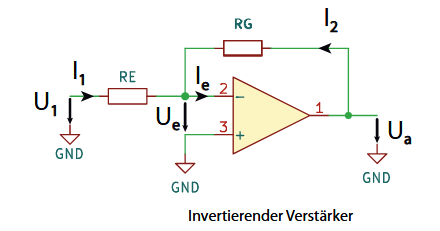
\includegraphics{graphics/invertierender Verstärker.png}}
    \caption{Schaltung: Invertierender Verstärker [Quelle: PAP2.2 Skript, S.30, Stand: 18.06.2024]}
    \label{fig:invVerstärker}
\end{figure}


\newpage
\subsubsection{Spannungsverstärkung des invertierenden Verstärkers}

Ausgehend von Abbildung \ref{fig:invVerstärker} kann man mit der Knotenregel die Ströme, die zum Eingang des Verstärkers fließen, identifizieren:

\begin{equation}
    I_1 + I_2 - I_e = 0
\end{equation}

Mit der Annahme eines hohen Innenwiderstands des Operationsverstärkers im Vergleich zu den Widerständen $R_1$ und $R_2$ kann man $I_e = 0$ nähern, woraus man dann mit der Leerlaufverstärkung $V_0 = U_a/U_e$ die folgende Form erhält:

\begin{equation}
    \begin{split}
        I_1 + I_2 &= \frac{U_1 - U_e}{R_1} + \frac{U_a - U_e}{R_2} = 0, \\ 
        \Rightarrow \frac{U_1}{U_a} &= - \left[ \frac{1}{V_0} + \frac{R_e}{R_g} \left( 1 + \frac{1}{V_0} \right) \right].
    \end{split}
\end{equation}

Bei dem von uns verwendeten Verstärker gilt $1/V_0 = 10^{-5} \ll 1$, weshalb man für den Fall, das $R_e/R_g$ groß gegenüber $1/V_0$ wird, die folgende Gleichung erhält:

\begin{equation}
    - \frac{U_a}{U_1} = \frac{R_g}{R_e} = V'.
    \label{eq:Betriebsverstärkung}
\end{equation}

Hierbei bezeichnet $U_a/U_1$ die Verstärkung des gekoppelten invertierten Verstärkers, welche somit in diesem Fall nur von der Außenbeschaltung und nicht von den Verstärkerdaten selbst abhängt. $V'$ wird somit auch Betriebsverstärkung genannt. Es ist zu beachten, dass diese Näherung nur solange gilt, wie die genannten Bedingungen weiterhin erfüllt bleiben. 

Wird in die Rückkopplung ein zusätzlicher Kondensator eingebaut, so koppeln höhere Frequenzen stärker als niedrigere und es entsteht ein Tiefpassverhalten. Das gegenteilige Hochpassverhalten erhält man beim Parallelschalten des Kondensators zu $R_e$.

\newpage
\subsection{Versuchsaufbau}

Der Aufbau besteht im Grunde aus drei Geräten: Einem Signalgenerator, welche die zu verstärkenden Eingangssignale liefert, dem Operationsverstärker $\mu$A 741, welcher wie in den Grundlagen erläutert funktioniert, und einem Zweikanal Oszilloskop zur Messung, Speicherung und Auslesung der Signale. Am Verstärker sind verschiedene Einstellungen für das Eingangssignal und die Rückkopplung des Ausgangssignals verfügbar. Zusätzlich ist in diesem direkt noch ein Gleichspannungsgenerator verbaut, welcher für den ersten Versuchsteil verwendet wird. Alle drei Geräte werden über Kabel dem Schaltkreis entsprechend verbunden.


\phantom{.}

\begin{figure}[!h]
    \centering
    \resizebox{0.9\textwidth}{!}{
    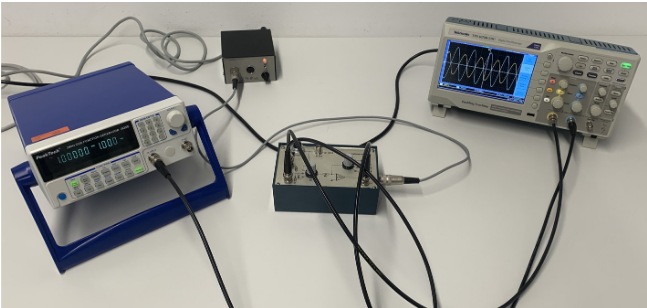
\includegraphics{graphics/aufbau.png}}
    \caption{Versuchsaufbau [Quelle: PAP2.2 Skript, S.28, Stand: 18.06.2024]}
    \label{fig:Aufbau}
\end{figure}




%---------------VERSUCHSPROTOKOLL MIT MESSDATEN---------------
\newpage

\section{Versuchsprotokoll mit Messdaten}

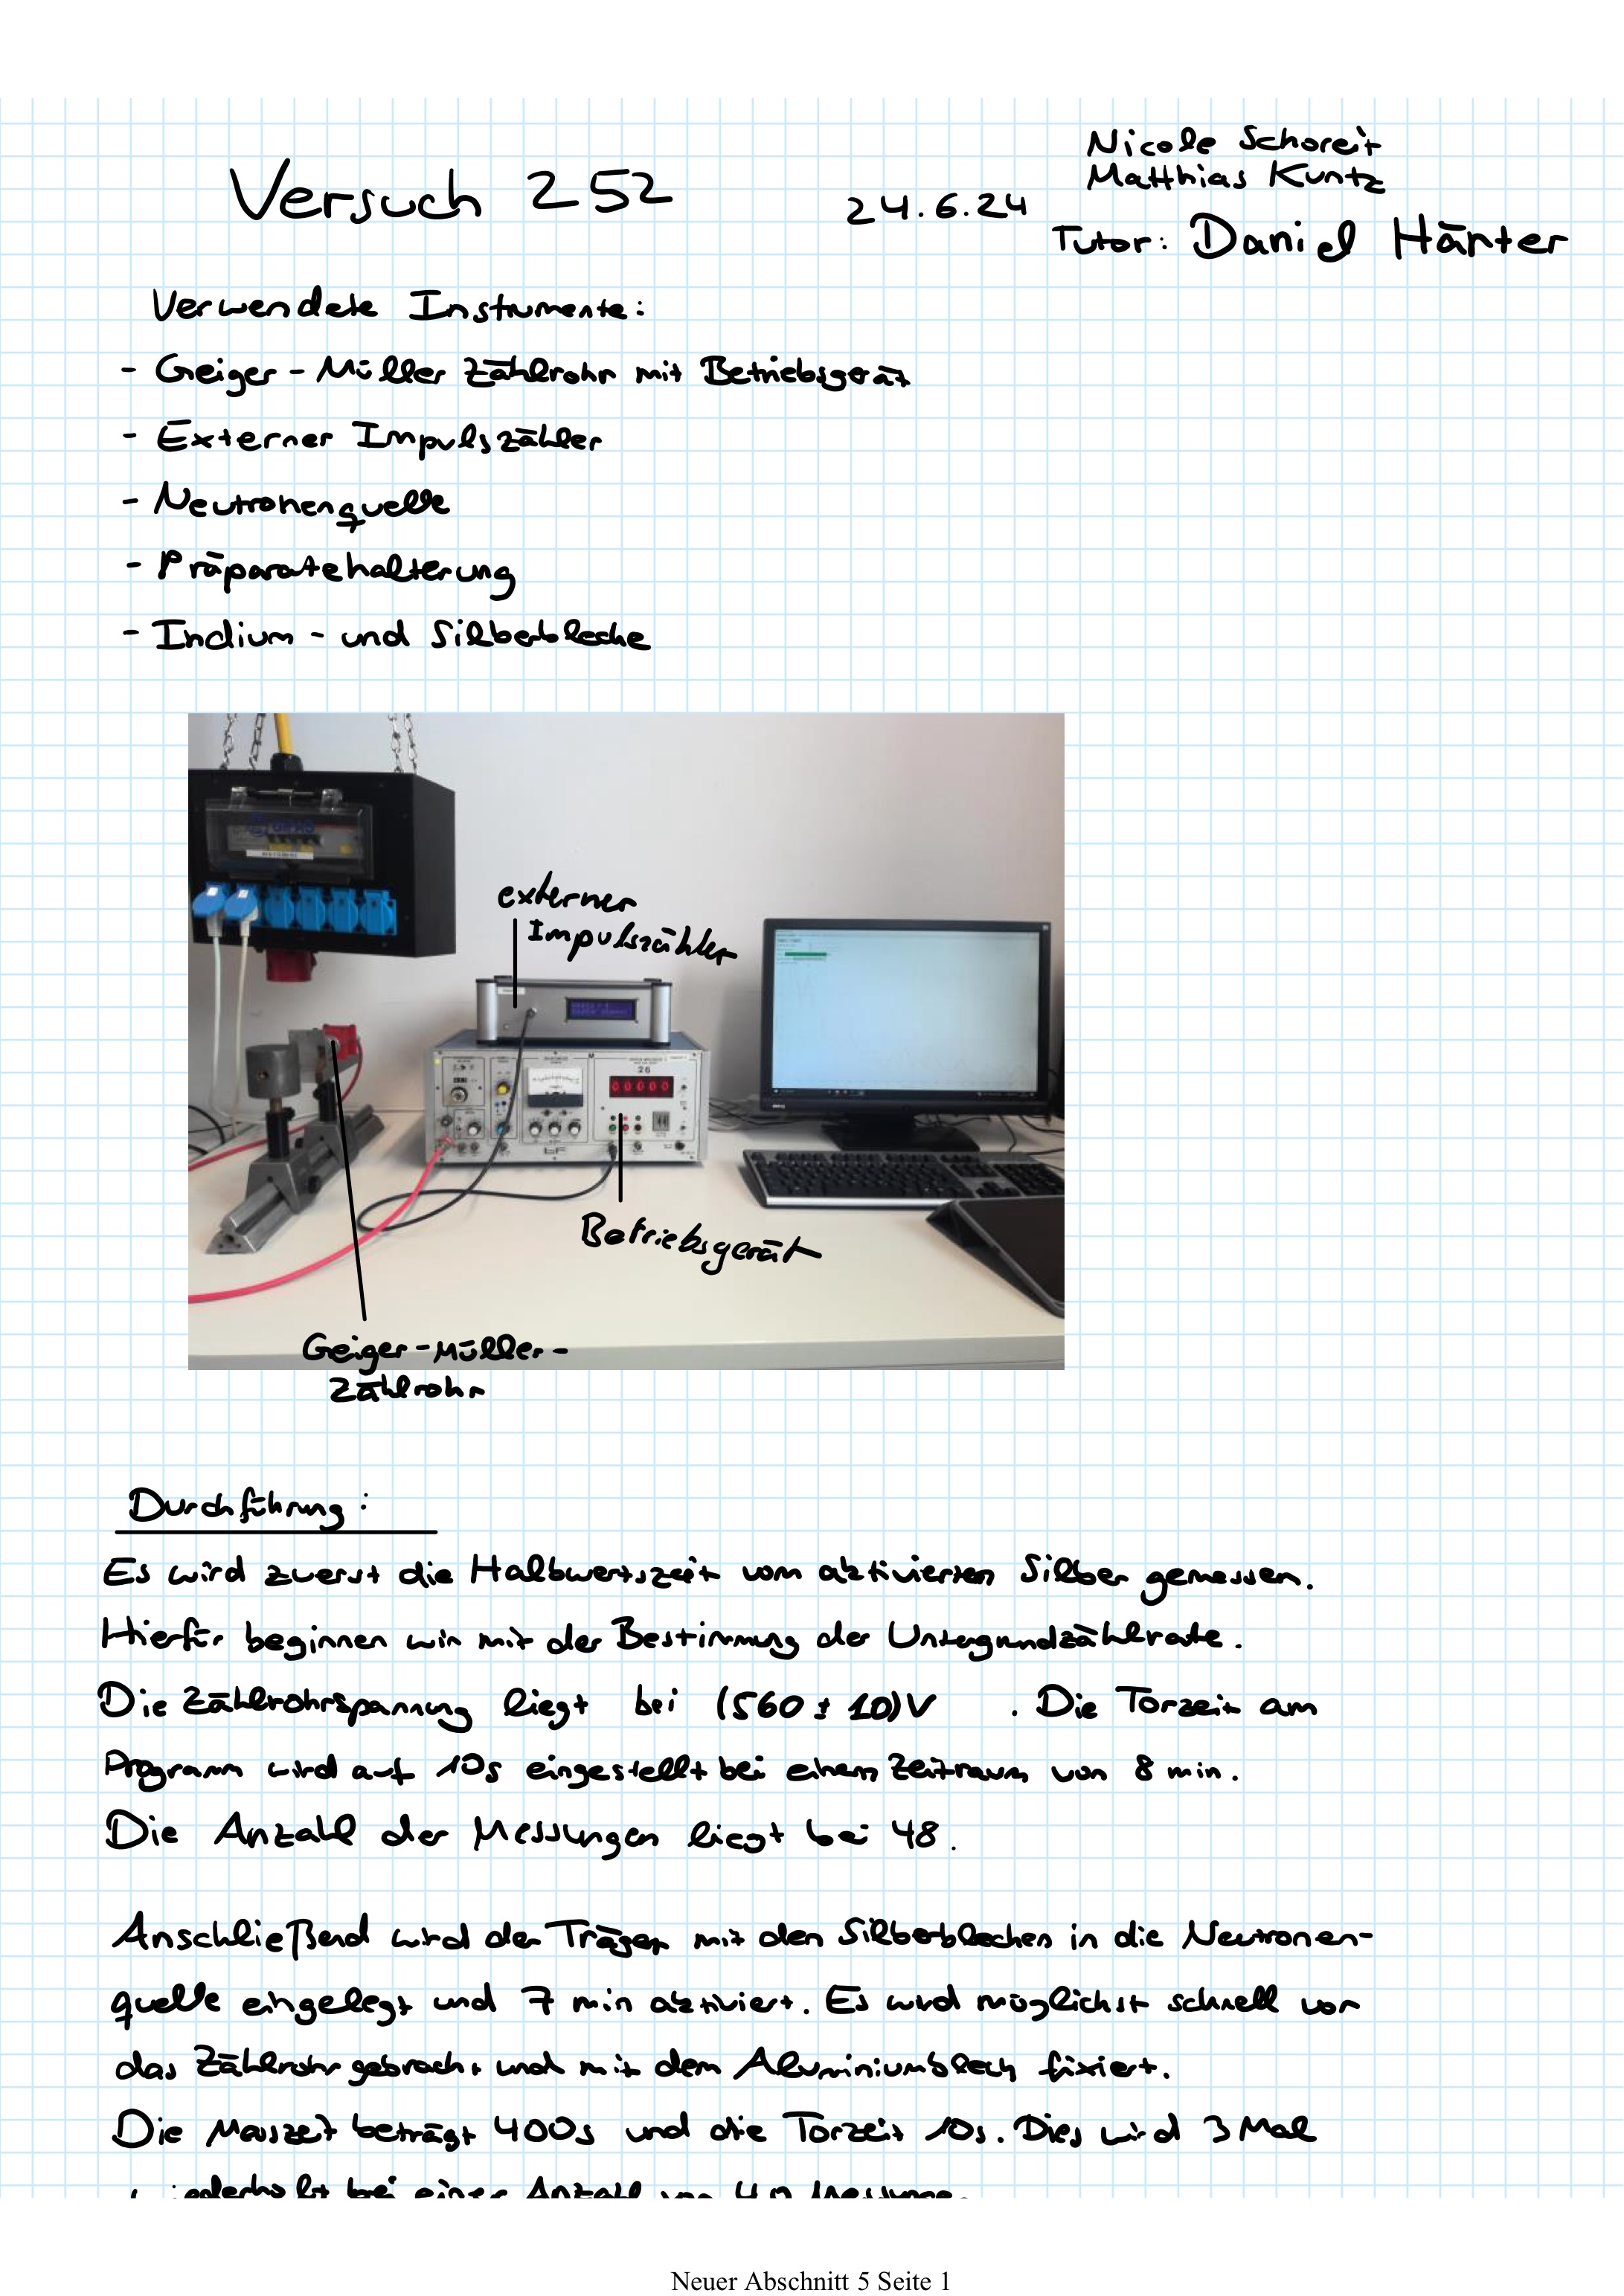
\includegraphics[width=\textwidth]{graphics/mess1.jpg}
\newpage

\includegraphics[width=\textwidth]{graphics/mess2.jpg}
\newpage
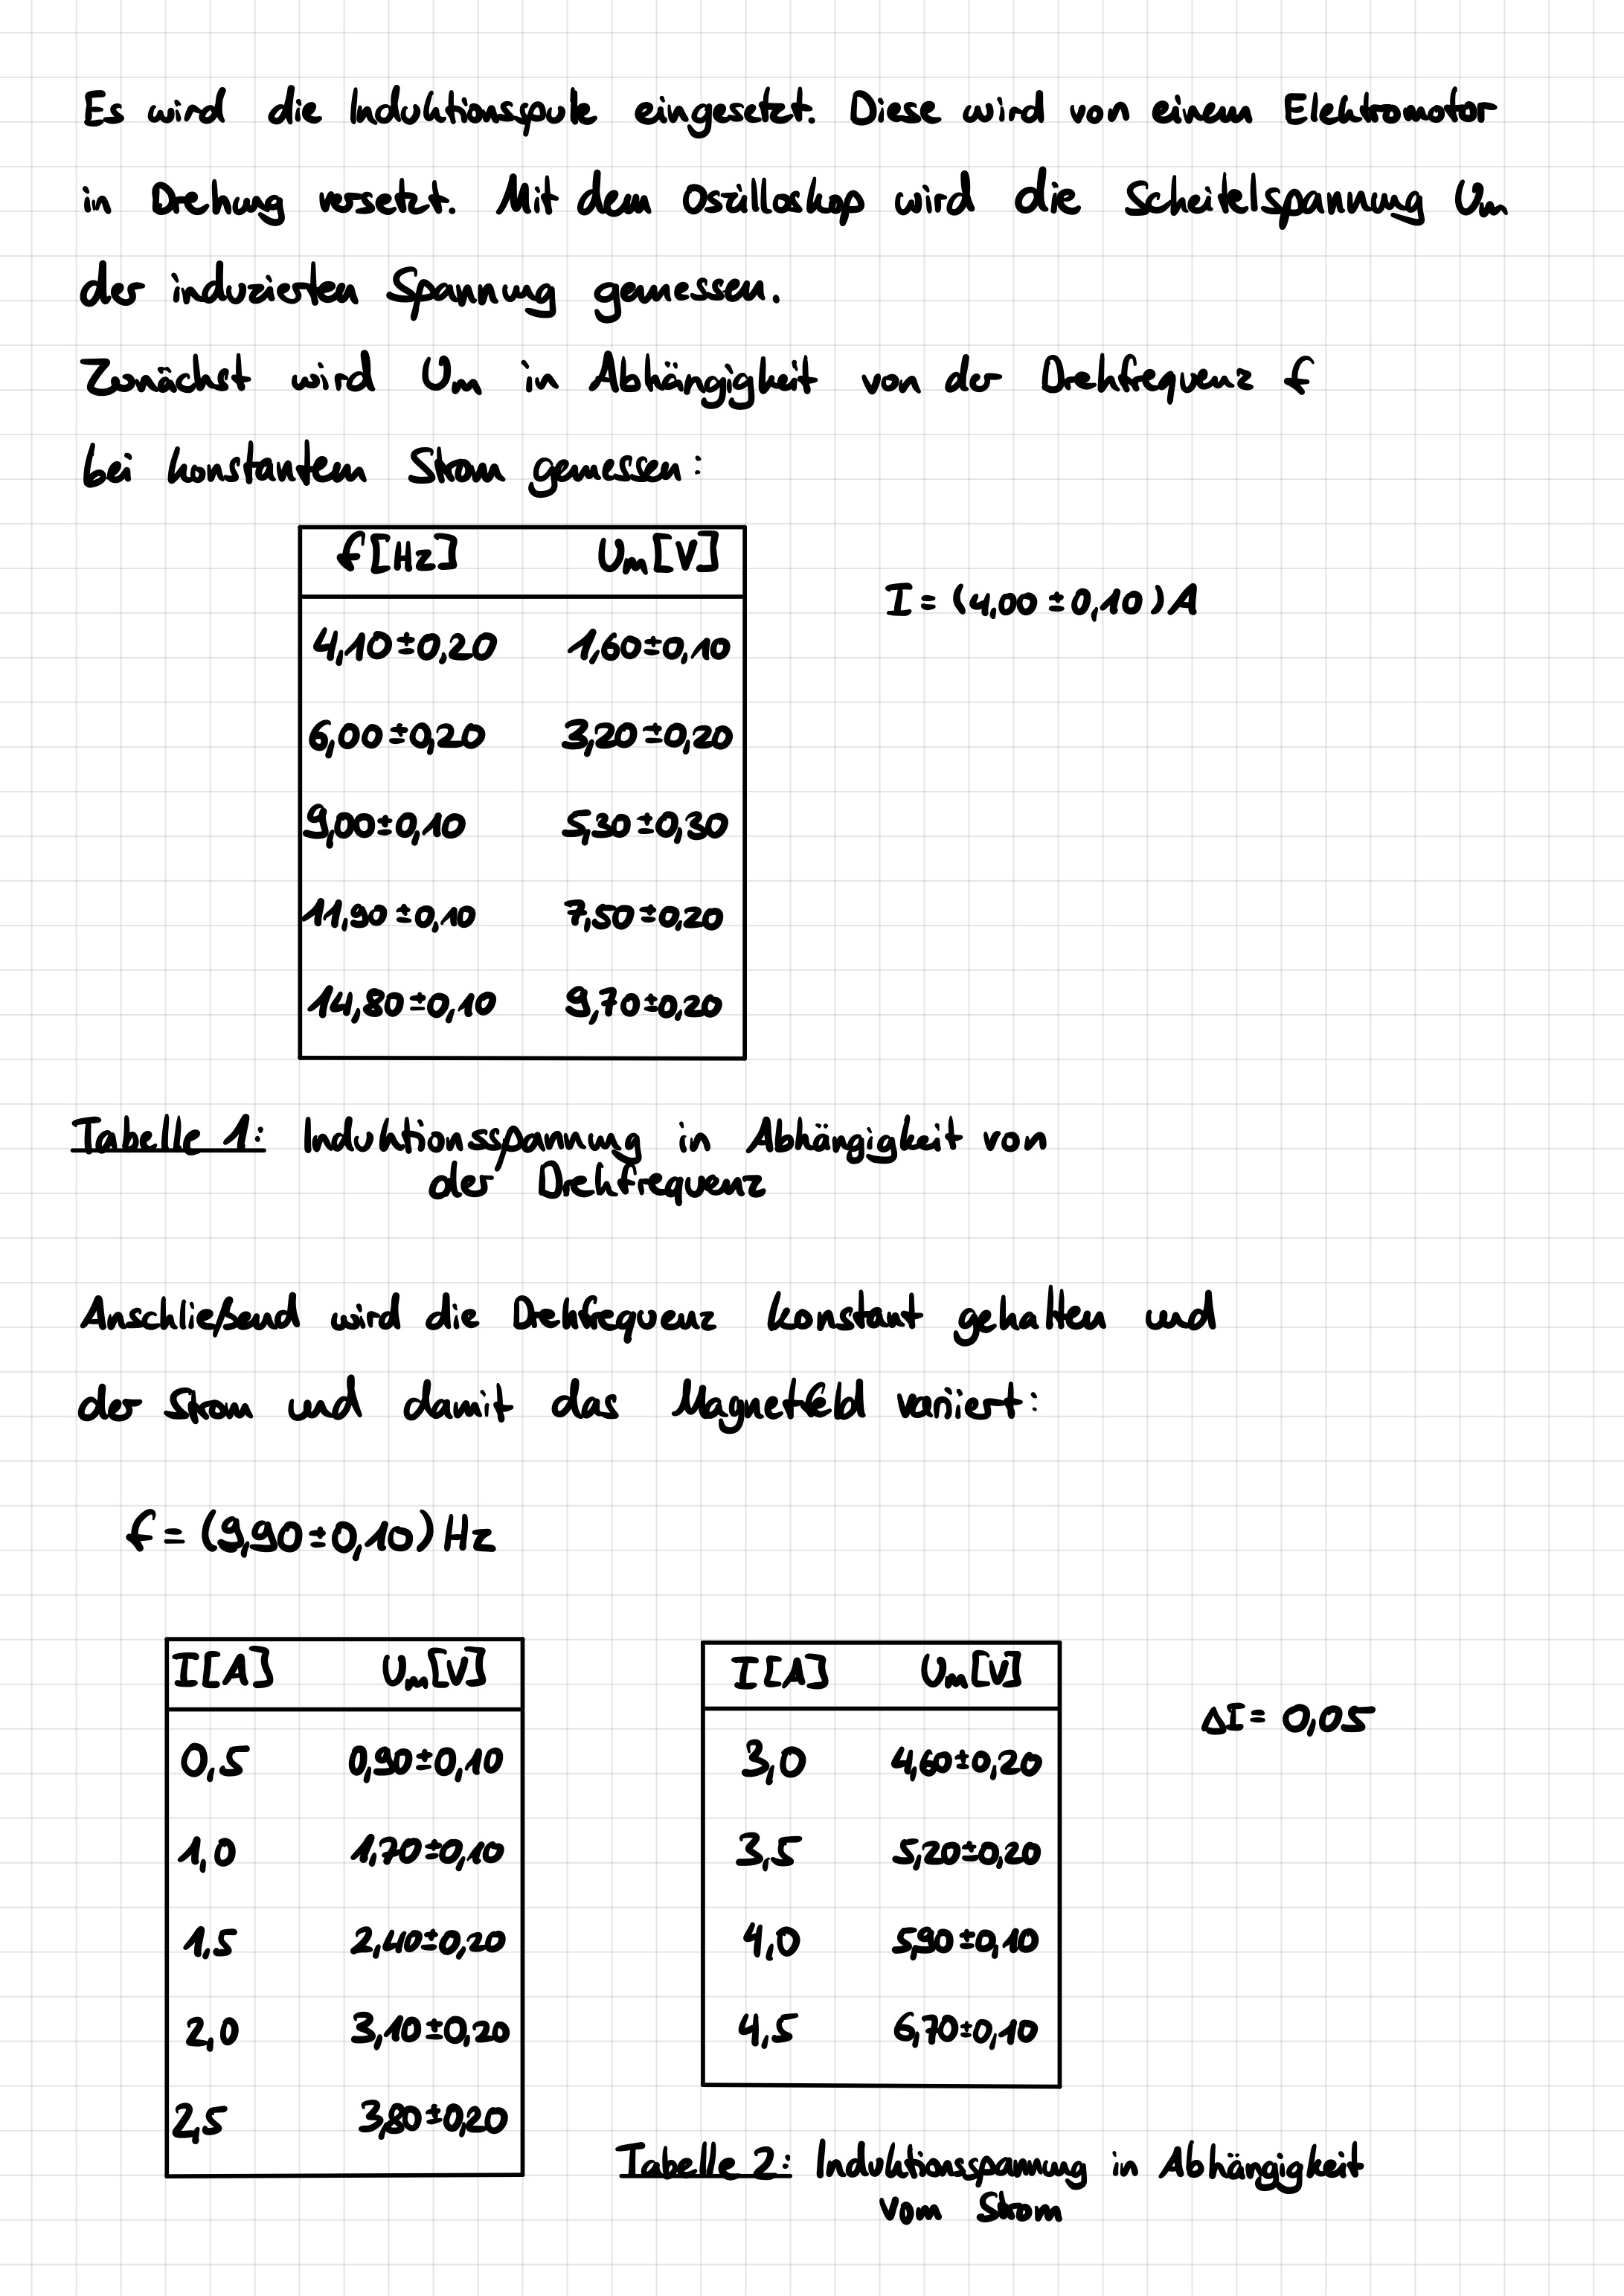
\includegraphics[width=\textwidth]{graphics/mess3.jpg}
\newpage
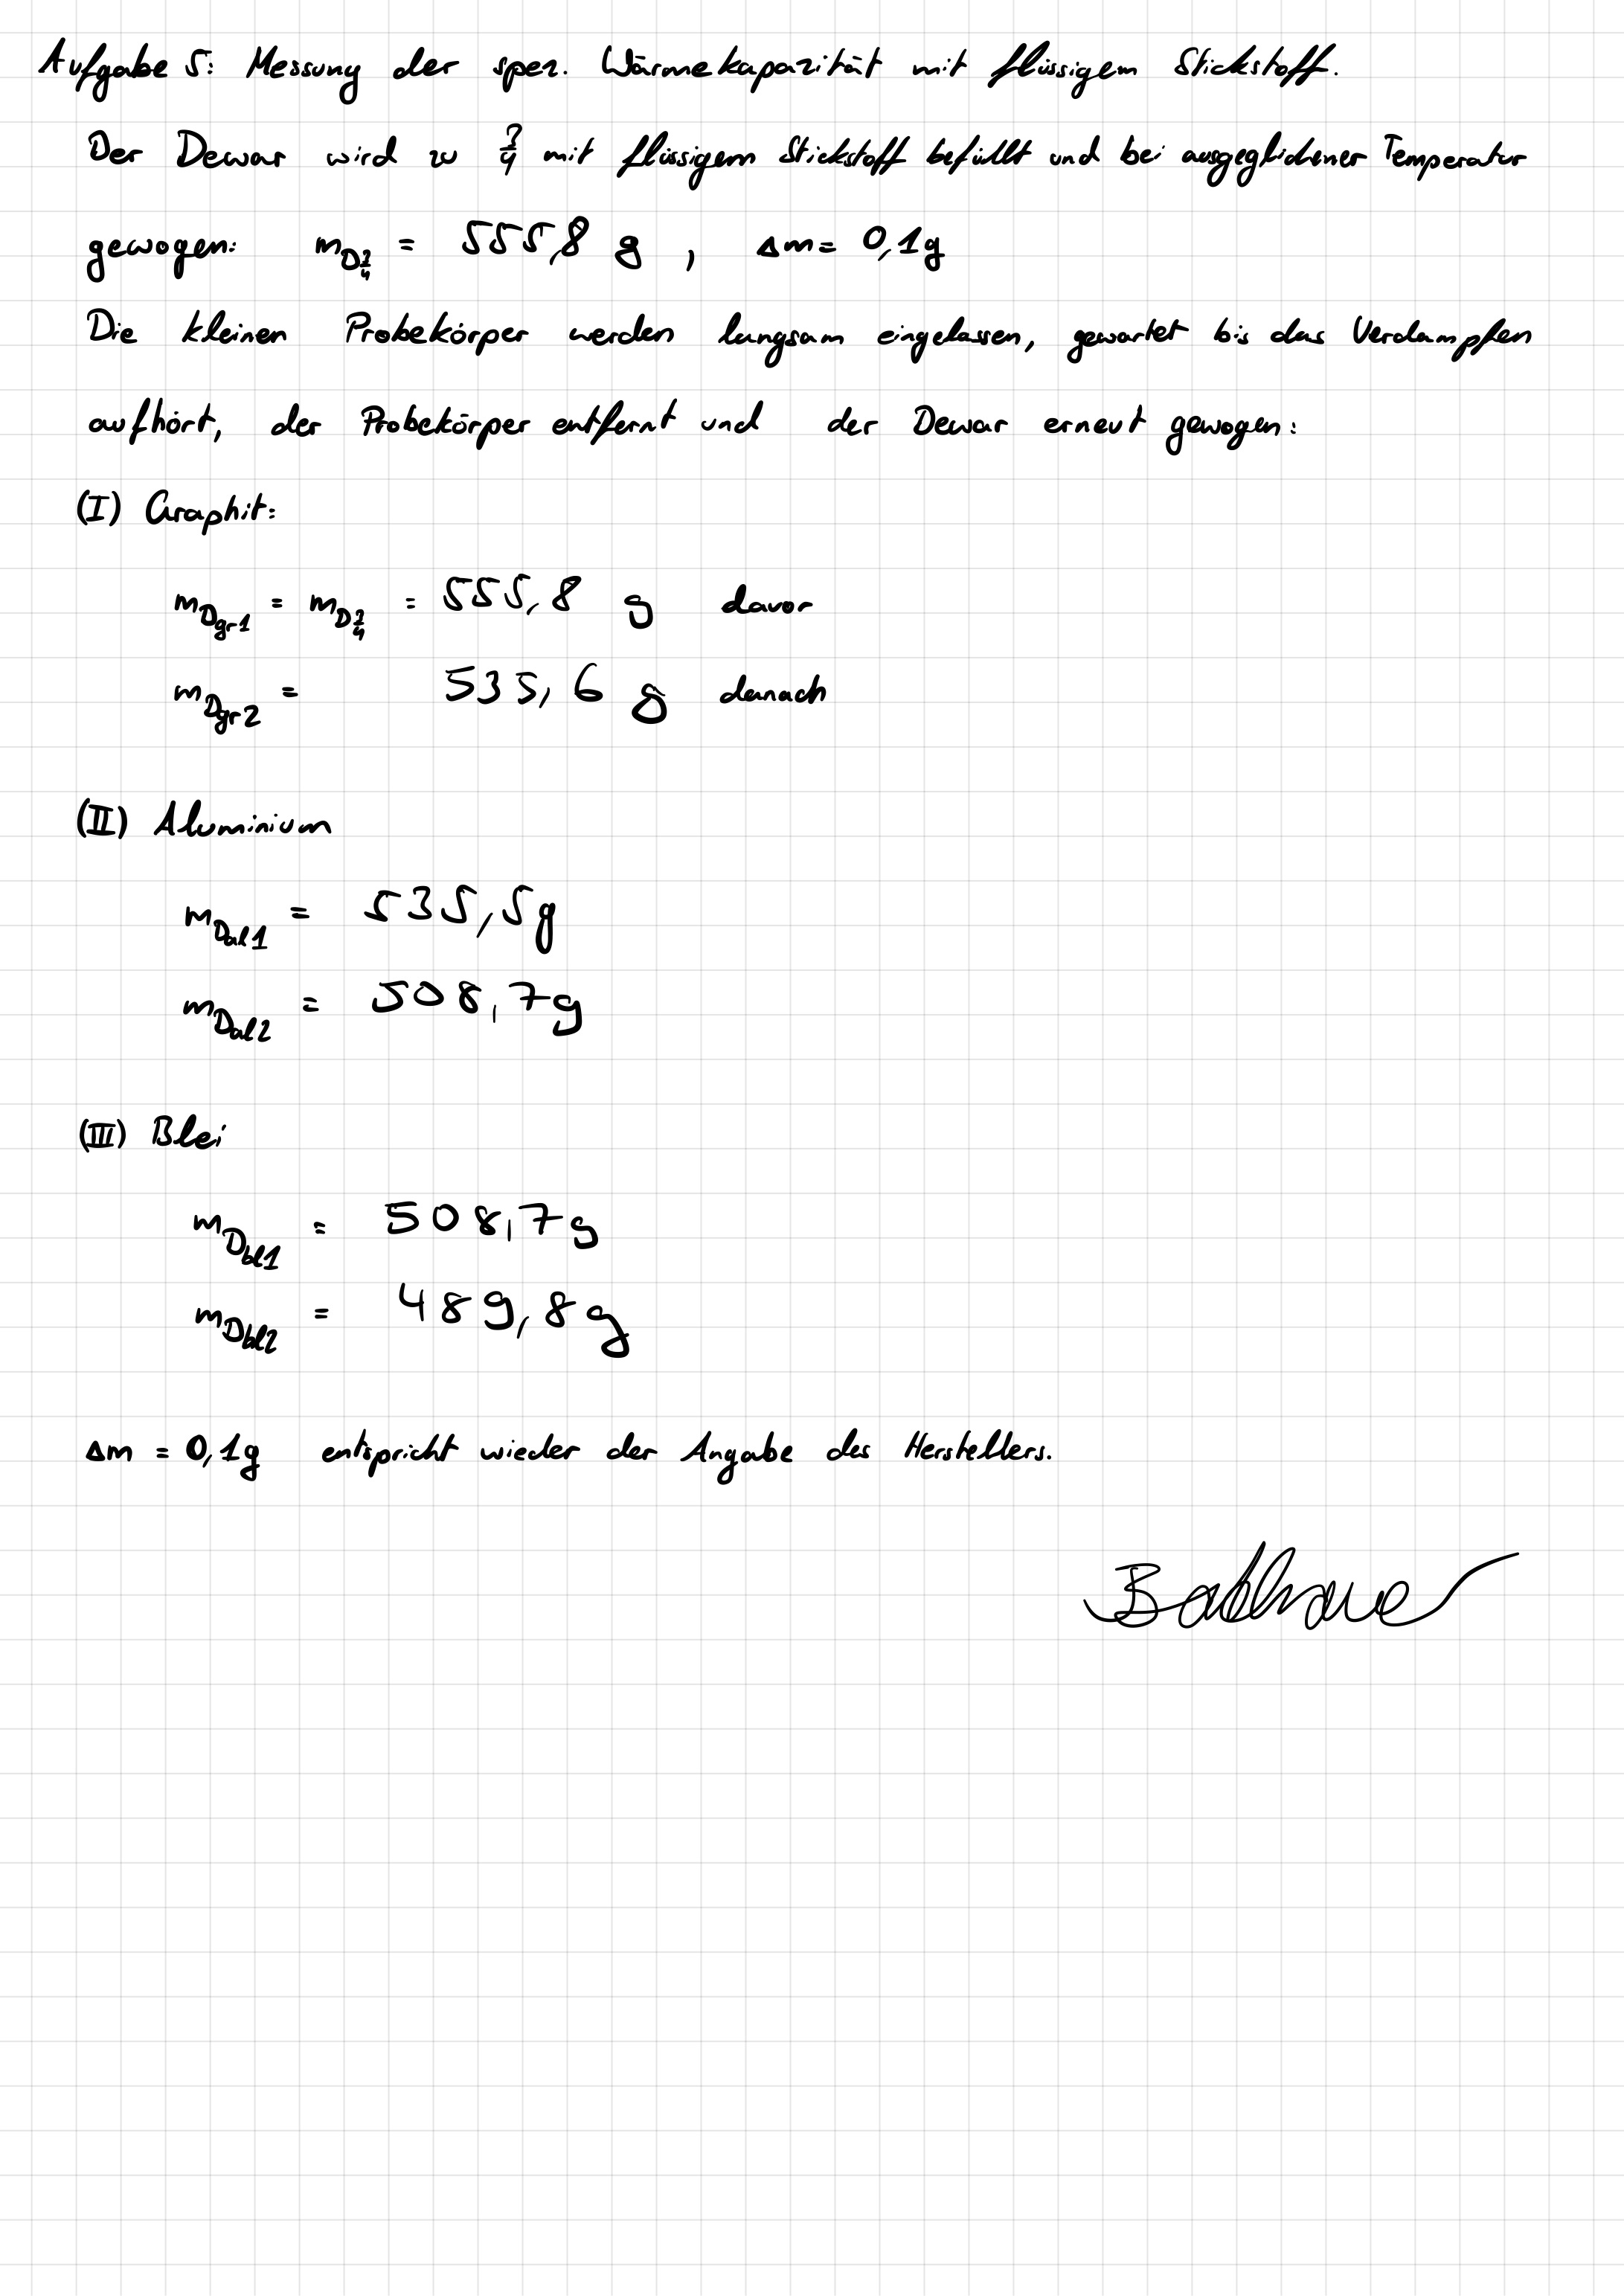
\includegraphics[width=\textwidth]{graphics/mess4.jpg}
\newpage
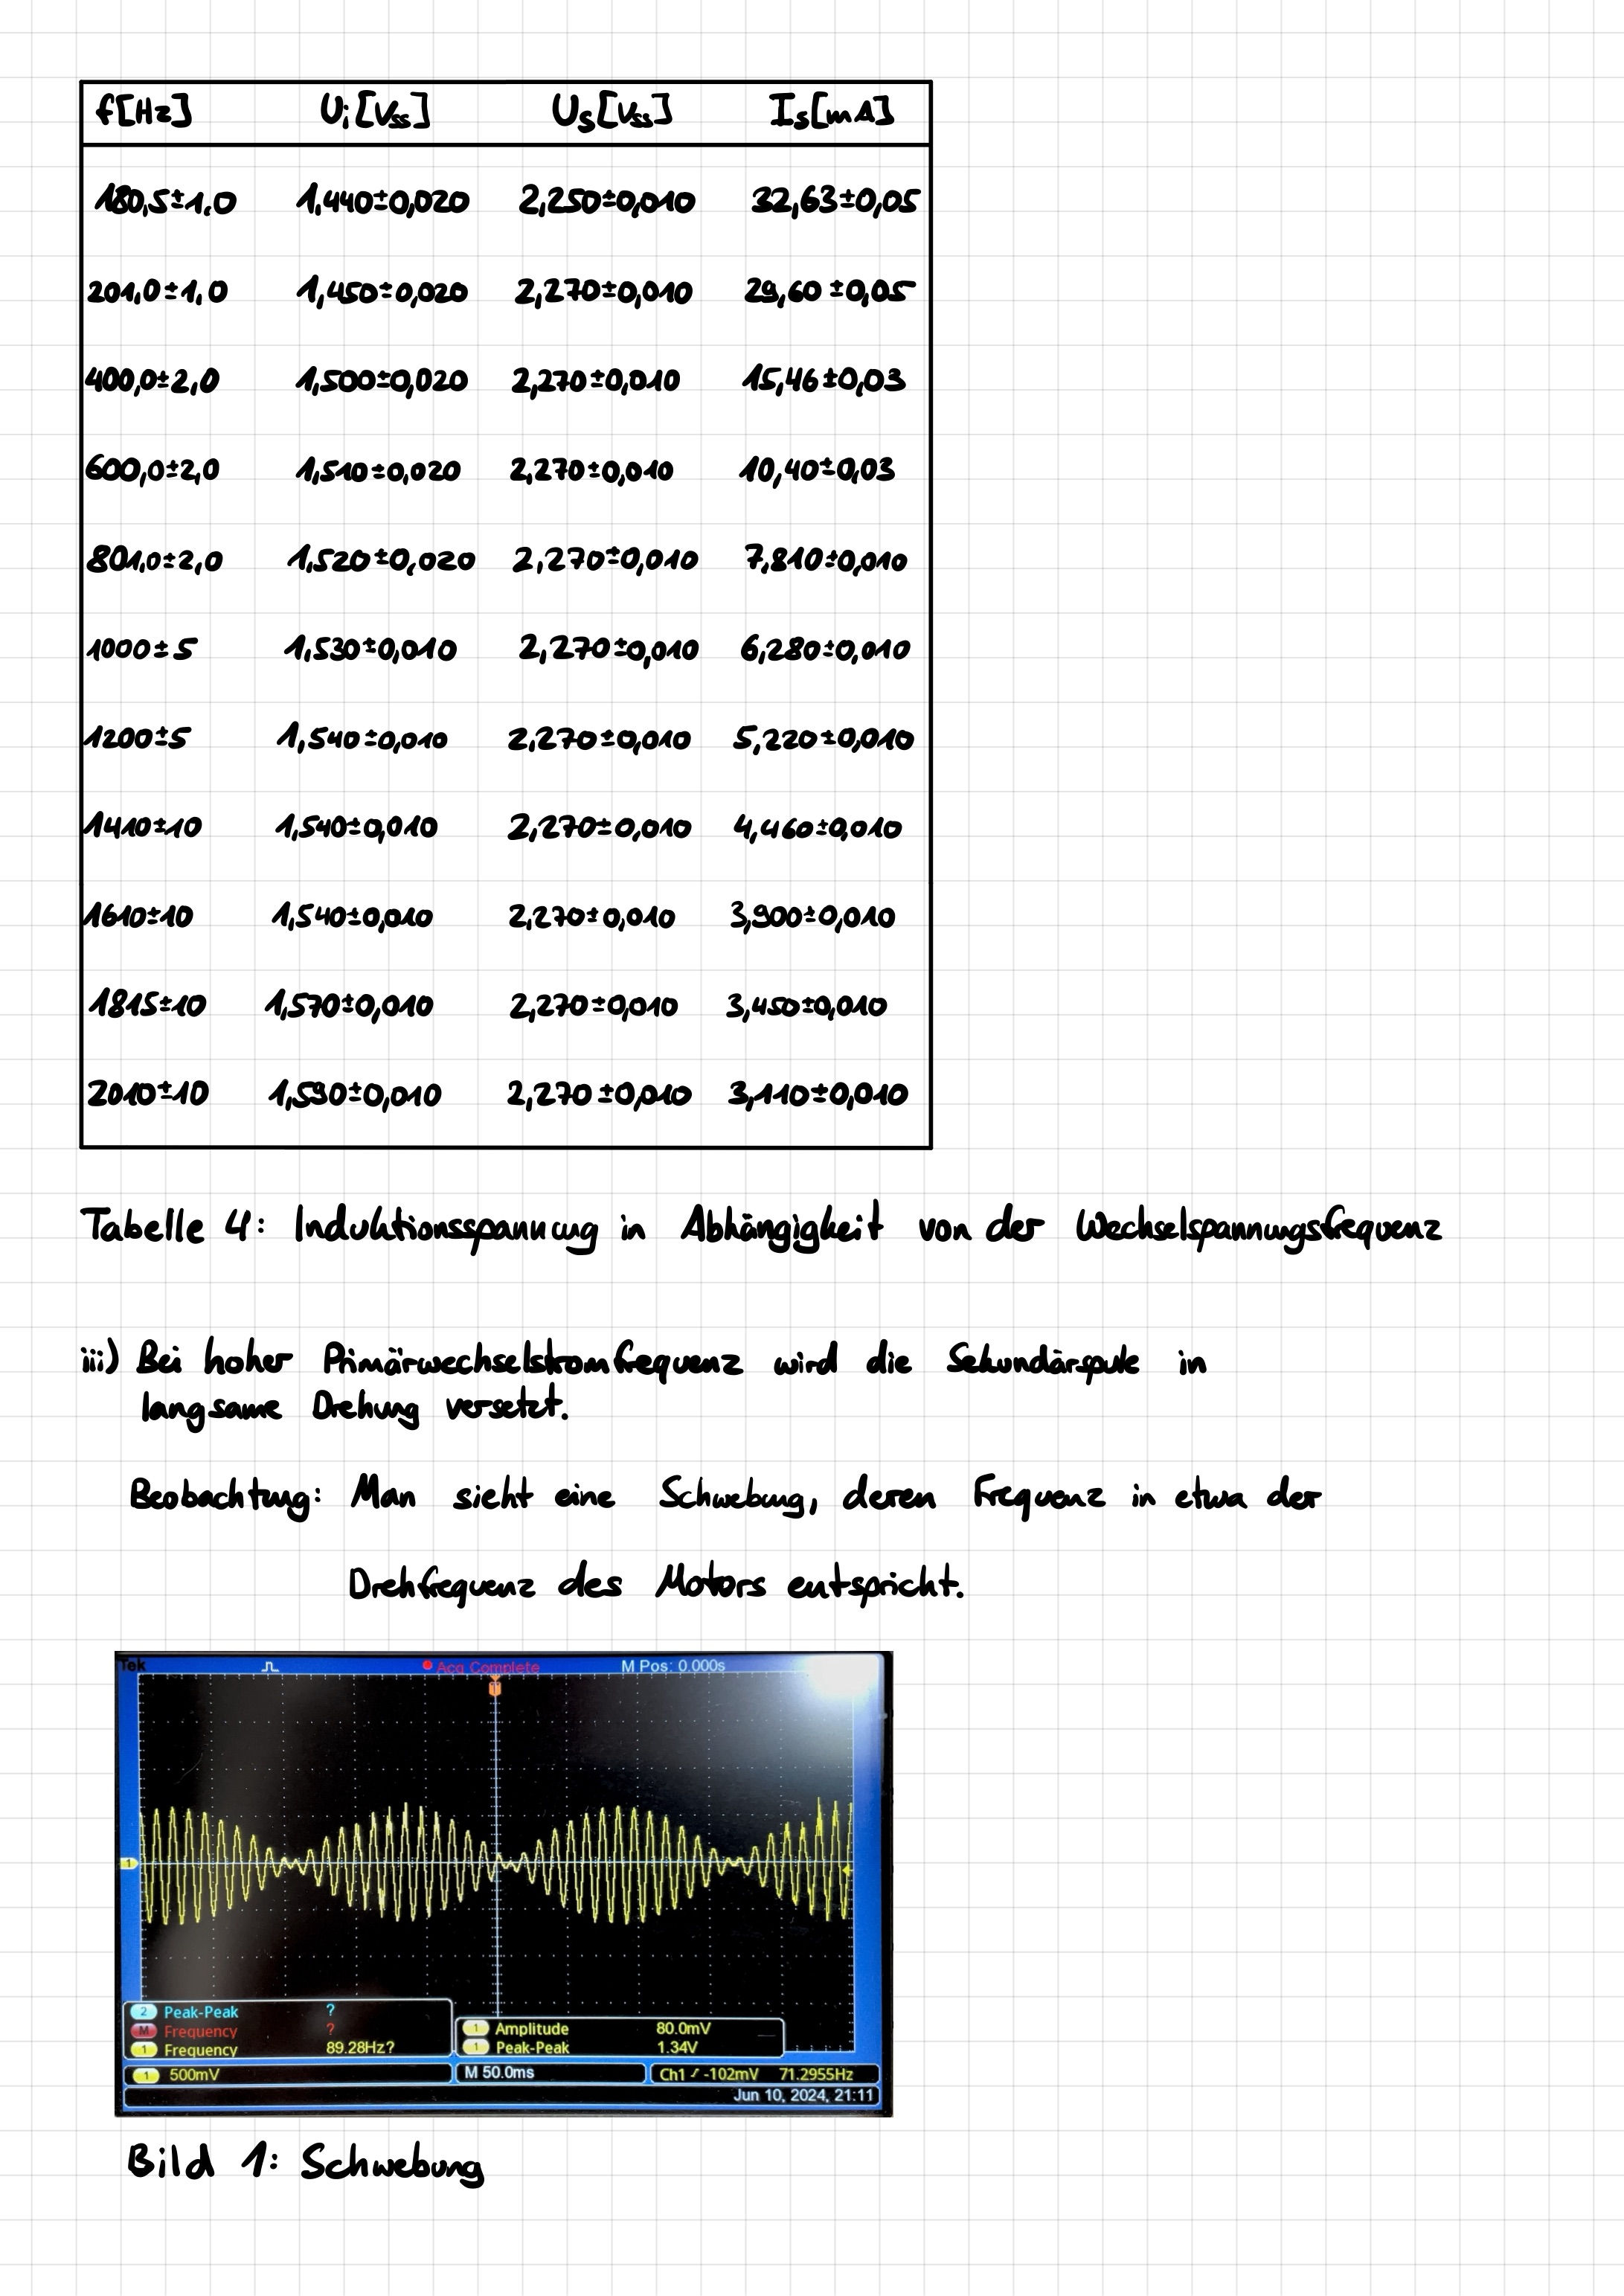
\includegraphics[width=\textwidth]{graphics/mess5.jpg}
\newpage
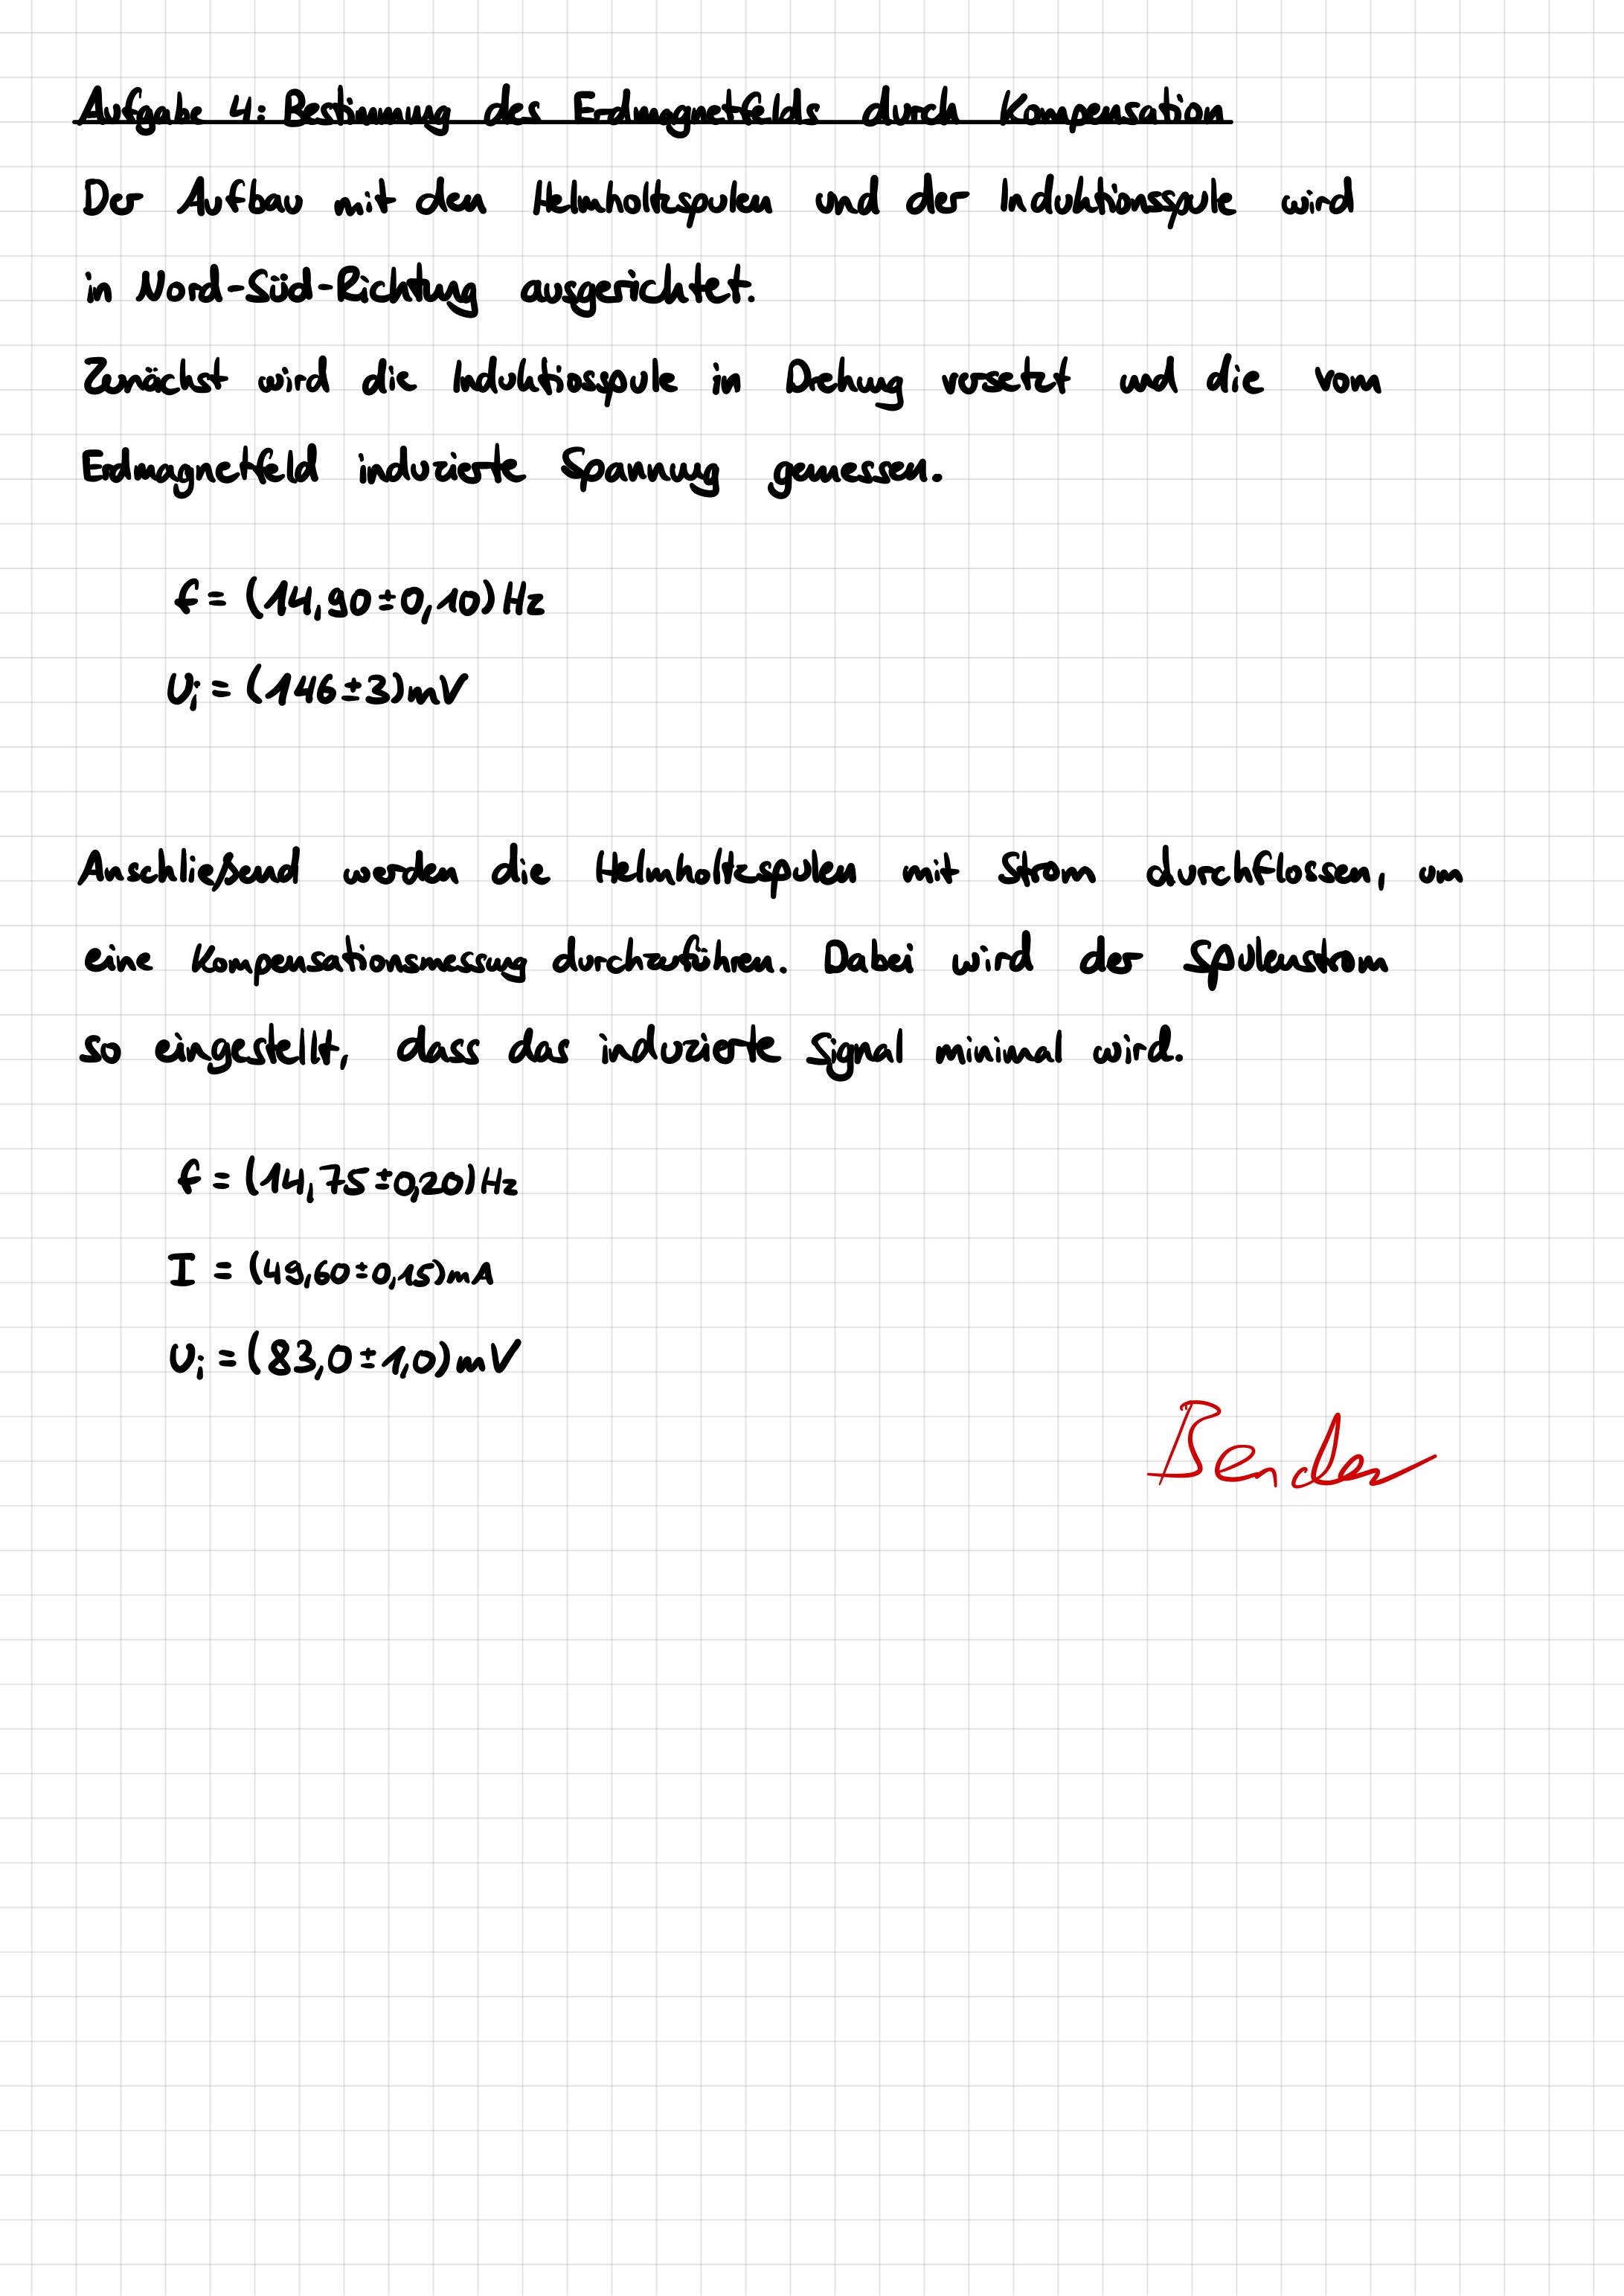
\includegraphics[width=\textwidth]{graphics/mess6.jpg}
\newpage
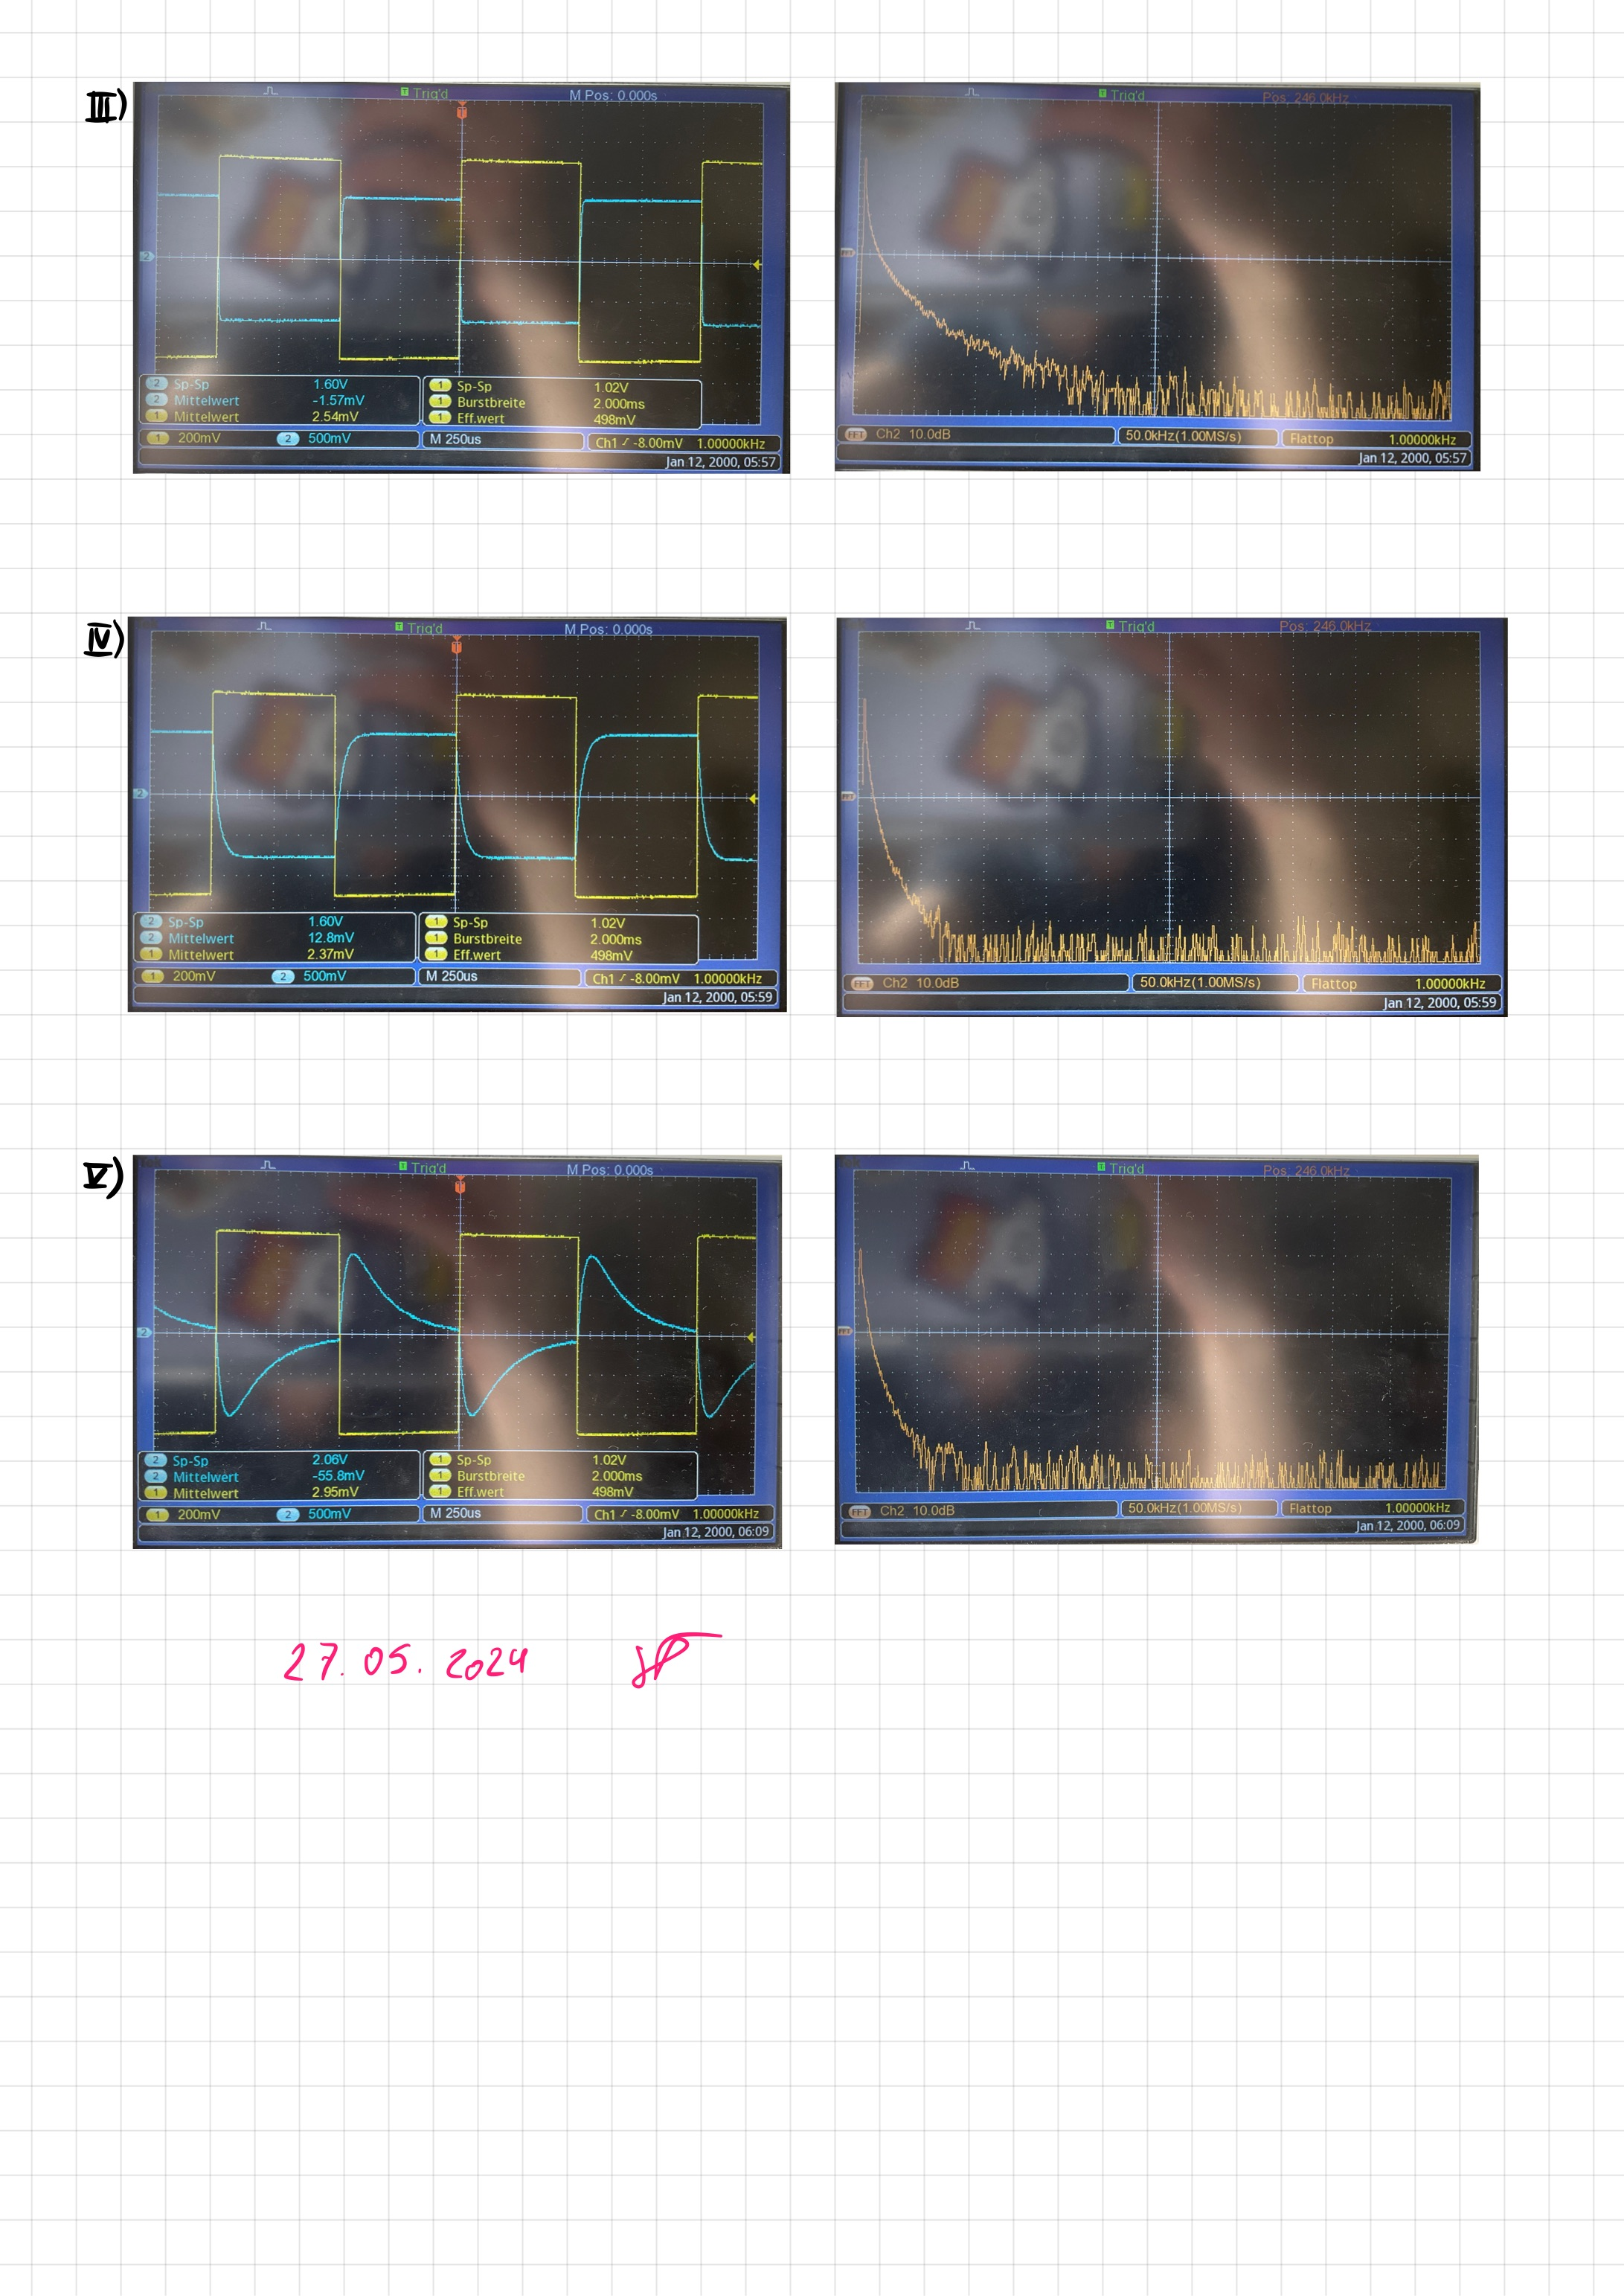
\includegraphics[width=\textwidth]{graphics/mess7.jpg}
\newpage

\addtocounter{table}{7}


\clearpage
\newpage
%-------------------------AUSWERTUNG-------------------------
\section{Auswertung}

In dieser Evaluation werden alle Fehler, sofern keine spezifische Angabe gemacht wird, mithilfe der Gauss'schen Fehlerfortpflanzung berechnet. Dies bedeutet, dass ein Wert $F$, der mit der Formel $f(a_1, ..., a_n)$ berechnet wird, den Fehler $\Delta F$ annimmt:

\begin{equation}
    \Delta F = \sqrt{\sum_n \left( \frac{\partial f}{\partial a_n} \cdot \Delta a_n \right)^2}.
\end{equation}

Des Weiteren erfolgen Signifikanztests von zwei Werten $a$ und $a'$ über die folgende Formel:

\begin{equation}
    \sigma = \frac{|a-a'|}{\sqrt{(\Delta a)^2 + (\Delta a')^2}}.
\end{equation}

Die Auswertung sowie Berechnung erfolgen über das dem Dokument angehängte Python-Programm. Hierbei erfolgen Fits von Funktionen mithilfe der 'curve\_fit'-Funktion des 'SciPy'-Packages und Plots werden mit 'matplotlib' erstellt.

Die Güte eines Fits wird mit der $\chi^2$-Summe bewertet:

\begin{equation}
    \chi^2 = \sum_i^N \left( \frac{\textit{Funktionswert}_i - \textit{Messwert}_i}{\textit{Fehler}_i} \right)^2
\end{equation}

Auch verwendet wird $\chi^2_{red} = \chi^2 / f$, wobei der Freiheitsgrad $f$ die Anzahl der Messwerte minus die Anzahl der Fitparameter ist. Der auf die Freiheitsgrade normierte Wert soll bei einem guten Fit ungefähr 1 sein.

\newpage

\subsection{Verstärkung von Gleich- und Wechselspannung}

Wir beginnen, indem wir unsere gemessenen Ausgangsspannungen aus Teil 1 des Messprotokolls für Gleich- und Wechselspannung in Diagramme über die Eingangsspannung auftragen. Bei den Wechselspannungen wird der Faktor 1/10 der Generatorspannung berücksichtigt. An die linearen Teile fitten wir jeweils Geraden $y = \alpha \cdot x + \beta$ an, wobei wir die in Tabelle \ref{tab:A1-Fitparameter} notierten Fitparameter für die jeweiligen Konfigurationen erhalten.

\phantom{.}

\begin{table}[!h]
    \centering
    %\resizebox{\textwidth}{!}{
    \begin{tabular}{cccc}
        \hline
        \textbf{Spannung} & $\bm{R_g}$ [k$\Omega$] & $\bm{\alpha}$ & $\bm{\beta}$ [V]  \\ \hline
         DC & 48,7 & -(16,3 $\pm$ 0,5) & 0,69 $\pm$ 0,07 \\
         DC & 274  & -(90,1 $\pm$ 0,8) & 1,39 $\pm$ 0,08 \\
         AC & 274  & 87,6 $\pm$ 0,3    & -(0,011 $\pm$ 0,016) \\
         AC & 680  & 194,2 $\pm$ 0,7   & -(0,200 $\pm$ 0,020) \\ \hline
    \end{tabular}%}
    \caption{Fitparameter der Linearen Fits}
    \label{tab:A1-Fitparameter}
\end{table}

\phantom{.}

Die Plots mit den Messdaten und jeweiligen Fits sind in den Abbildungen \ref{fig:A1_gleichspannung} \& \ref{fig:A1_wechselspannung} zu sehen. Zur qualitativen Bewertung der Fits berechnen wir für alle vier die $\chi^2$-Werte und die Fitwahrscheinlichkeit.

\phantom{.}

\begin{table}[!h]
    \centering
    %\resizebox{\textwidth}{!}{
    \begin{tabular}{ccccc}
        \hline
        \textbf{Spannung} & $\bm{R_g}$ [k$\Omega$] & $\bm{\chi^2}$ & $\bm{\chi^2_{red}}$ & \textbf{Wsk.} [\%] \\ \hline
         DC & 48,7 & 0,26 & 0,04 & 100  \\
         DC & 274  & 3,71 & 0,74 & 59,0  \\
         AC & 274  & 10,07 & 2,52 & 4,0  \\
         AC & 680  & 331,33 & 82,83 & 0,0  \\ \hline
    \end{tabular}%}
    \caption{Fitbewertung}
    \label{tab:A1-Fitbewertung}
\end{table}

\phantom{.}

Wie gut zu erkennen ist, werden die Fits zunehmend inakkurater. Hier lassen sich auf die letzten beiden Fits bezogene Fehlerquellen in der Analyse von Wechselspannung vermuten. Allgemein lässt sich sagen, dass bei den ersten beiden Fits die Fehler zu groß und bei den letzten Beiden zu klein abgeschätzt wurden, was auch gut in den Plots zu erkennen ist. Bei den Wechselspannungen weichen insbesondere die Werte bei höheren Generatorspannungen mehr vom Fit ab, was für die hohen $\chi^2$-Summen sorgt.

Bei den Fits entsprechen die Steigungen $\alpha$ nach Gleichung \ref{eq:Betriebsverstärkung} genau der Betriebsverstärkung $V'$, wobei das Vorzeichen zu beachten ist. Die theoretischen Werte zum Vergleich berechnen sich, ebenso in Gleichung \ref{eq:Betriebsverstärkung} zu sehen, aus dem Verhältnis vom eingestellten Rückkopplungswiderstand $R_g$ zum Eingangswiderstand $R_e$, welcher bei unserem Operationsverstärker 3k$\Omega$ beträgt. Die Fehler berechnen sich somit mit der gegebenen Toleranz von 10\% der Widerstände folgendermaßen:

\begin{equation}
    \Delta V'_{theo} = V'_{theo} \sqrt{2 \cdot 0,1^2}
\end{equation}

Die experimentell bestimmten und theoretischen Werte für die Betriebsverstärkung $V'$ sind mitsamt Signifikanztests in Tabelle \ref{tab:A1-Betriebsverstärkung} dargestellt.

\phantom{.}

\begin{table}[!h]
    \centering
    %\resizebox{\textwidth}{!}{
    \begin{tabular}{ccccc}
        \hline
        \textbf{Spannung} & $\bm{R_g}$ [k$\Omega$] & $\bm{V'_{exp}}$ & $\bm{V'_{theo}}$ & $\bm{\sigma}$  \\ \hline
         DC & 48,7 & 16,3 $\pm$ 0,5  & 16,2 $\pm$ 2,3 & 0,03 \\
         DC & 274  & 90,1 $\pm$ 0,8  & 91 $\pm$ 13 & 0,10 \\
         AC & 274  & 87,6 $\pm$ 0,3  & 91 $\pm$ 13 & 0,29 \\
         AC & 680  & 194,2 $\pm$ 0,7 & (0,23 $\pm$ 0,03)$\cdot 10^{3}$ & 1,01 \\ \hline
    \end{tabular}%}
    \caption{Experimentell und theoretisch bestimmte Betriebsverstärkung}
    \label{tab:A1-Betriebsverstärkung}
\end{table}

\phantom{.}

Man beobachtet wie erwartet, dass die Betriebsverstärkung für höhere Rückkopplungswiderstände zunimmt und theoretisch bei Gleich- und Wechselspannung ein gleiches Verhalten aufweist. Zwar weichen die beiden Werte bei $R_g = 274$ k$\Omega$ bei uns leicht ab, allerdings nur innerhalb der Fehler. 

Insgesamt sind keine signifikanten Abweichungen festzustellen. Jedoch ist anzumerken, dass die theoretischen Werte durch die recht hohe Toleranz von 10\% auch einen entsprechend erhöhten Fehler im Vergleich zu den Messwerten aufweisen und somit die Signifikanztests sehr positiv ausfallen.  

\begin{figure}[!p]
  \centering
  \subfloat[$R_g = 48,7$ k$\Omega$]{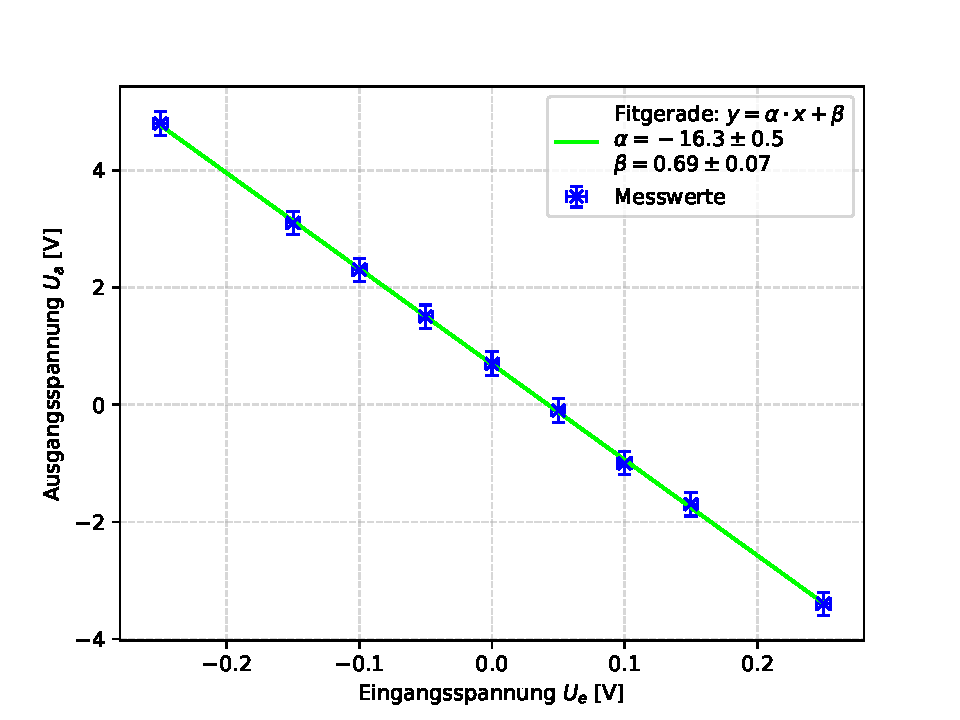
\includegraphics[width=0.9\textwidth]{graphics/plots/A1-DC48.pdf}}
  \hfill
  \subfloat[$R_g = 274$ k$\Omega$]{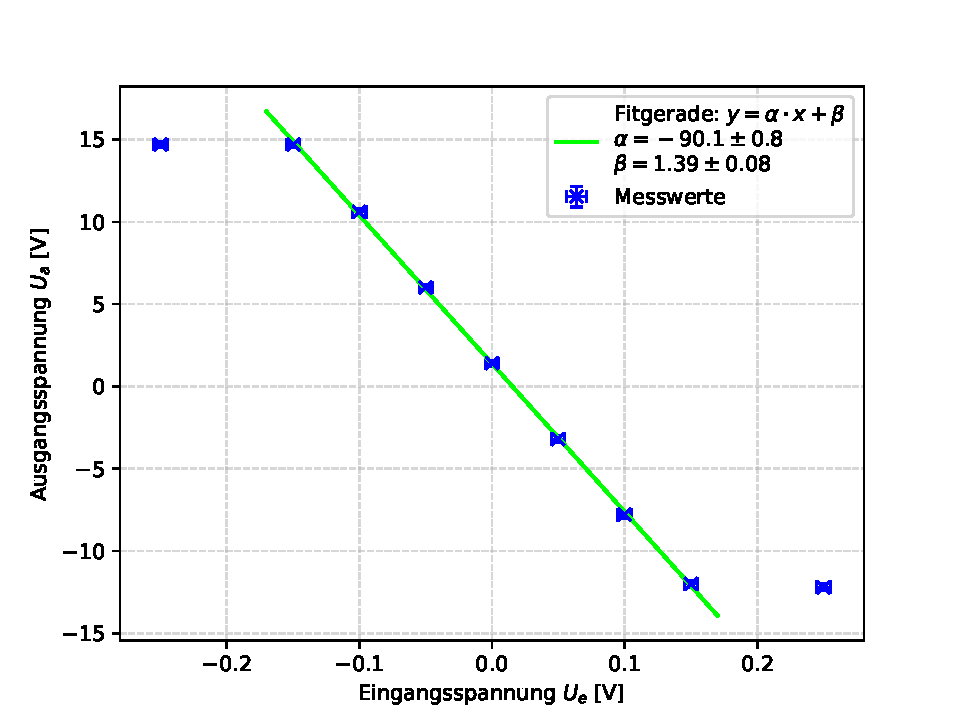
\includegraphics[width=0.9\textwidth]{graphics/plots/A1-DC274.pdf}}
  \hfill
  \caption{A1 - $U_a$ gegen $U_e$ - Gleichspannung}
  \label{fig:A1_gleichspannung}
\end{figure}

\begin{figure}[!p]
  \centering
  \subfloat[$R_g = 274$ k$\Omega$]{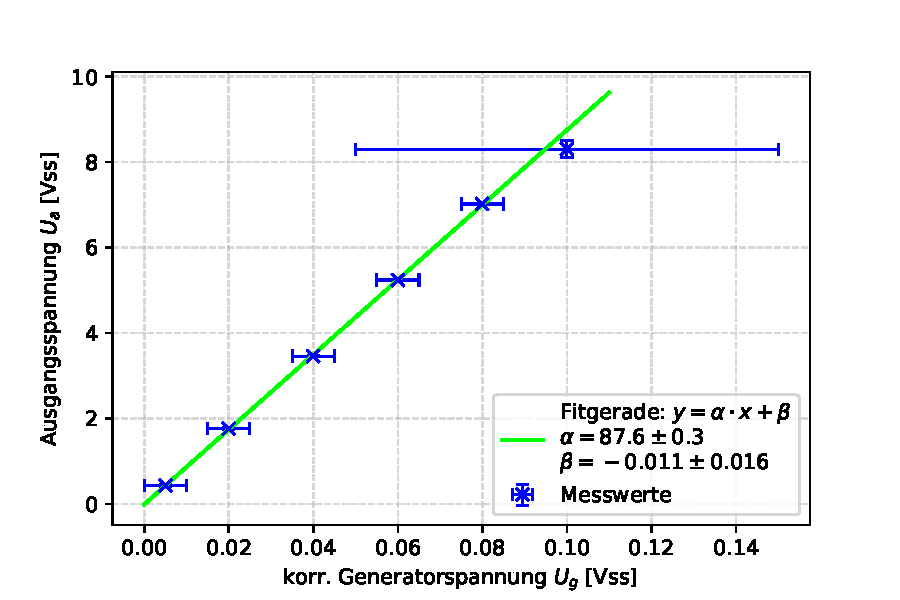
\includegraphics[width=0.9\textwidth]{graphics/plots/A1-AC274.pdf}}
  \hfill
  \subfloat[$R_g = 680$ k$\Omega$]{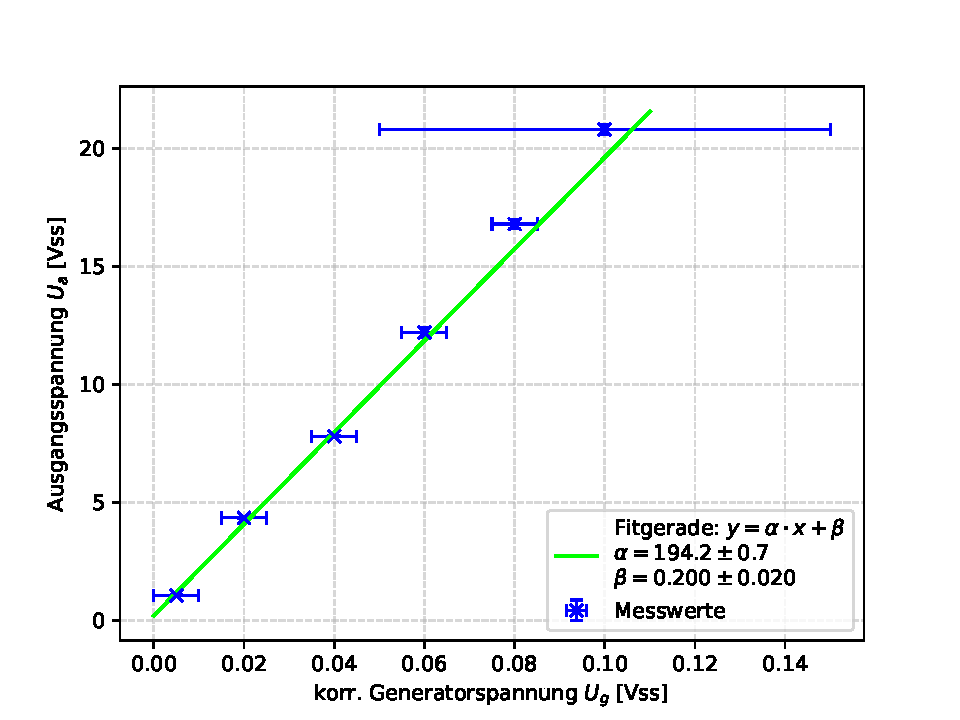
\includegraphics[width=0.9\textwidth]{graphics/plots/A1-AC680.pdf}}
  \hfill
  \caption{A1 - $U_a$ gegen $U_e$ - Wechselspannung}
  \label{fig:A1_wechselspannung}
\end{figure}

\clearpage
\newpage
\subsection{Frequenzgänge verschiedener Verstärkerkonfigurationen}

Wir stellen unsere in Teil 2 des Messprotokolls gemessenen Ausgangsspannungen in doppellogarithmischen Plots gegen die Frequenz dar. Die Messreihen aus Tabelle 5 sind alle in Abbildung \ref{fig:A2_1} dargestellt, der Frequenzgang aus Tabelle 6 mit parallel geschaltetem Gegenwiderstand ist in Abbildung \ref{fig:A2_2} und der letzte Frequenzgang aus Tabelle 7 mit Eingangshochpassfilter ist in Abbildung \ref{fig:A2_3} zu sehen. Um den Verlauf besser bewerten zu können fitten wir an die Messreihen die theoretischen Verläufe an. Diese entsprechen bei den Messreihen aus den Tabellen 5 \& 6 der Form

\begin{equation}
    y = \left[ \alpha \cdot x^\beta + \gamma \right]^{-1}
\end{equation}

und bei der letzten Messung mit Eingangshochpassfilter kommt ein Background-Offset dazu

\begin{equation}
    y = bkg - \left[ \alpha \cdot x^\beta + \gamma \right]^{-1}.
\end{equation}

Somit erhalten wir die in den Abbildungen \ref{fig:A2_1} bis \ref{fig:A2_3} ebenso dargestellten Fits.

Wenn wir die Verläufe der in Serie geschalteten Gegenwiderstände betrachten so kann man erkennen, dass die Messreihen wie theoretisch erwartet für hohe Frequenzen annähernd gleich verlaufen. Insbesondere der grüne und blaue Fit verlaufen recht ähnlich. Die etwas größere Abweichung beim roten Fit kann von der bereits niedrigen Spannung bei kleinen Frequenzen durch den geringeren Rückkopplungswiderstand stammen. Insgesamt zeigt sich aber der erwartete Verlauf und man erkennt, wie sich die drei Verläufe für hohe Frequenzen dem Verlauf der Leerlaufverstärkung annähern. Allgemein lassen sich Abweichungen zwischen den drei Fits wohl auf leichte Schwankungen in der Leerlaufverstärkung zurückschließen, die somit für leicht verschiedenen Verläufe bei hohen Frequenzen sorgen. 

Ein ähnliches Bild ist bei der Messreihe mit parallel geschaltetem Rückkopplungswiderstand erkennbar. Auch hier geht der Verlauf für höhere Frequenzen in einen eher konstanten Abfall über. Somit nähert er sich hier ebenso der Leerlaufverstärkung an.

Die Messreihe bei vorgeschaltetem Eingangshochpassfilter zeigt im aufgenommenen Frequenzbereich das erwartete Hochpassverhalten. Signale bei niedrigen Frequenzen werden abgeschwächt und nur die bei hohen ganz durchgelassen. Es ist zu beachten, dass die Messwerte hier nur bis zu einer Frequenz etwas über 10$^{4}$ gehen und somit der Teil, in dem sich der Verlauf der Leerlaufverstärkung annähert, noch nicht ganz erreicht wird. Der bisher immer beobachtete charakteristische Abfall bei hohen Frequenzen ist somit außerhalb des aufgenommenen Bereichs und lässt sich nur am leichten Abfall der letzten zwei Messpunkte vorahnen. 

Insgesamt zeigen die Plots somit die erwarteten Verläufe für alle Frequenzgänge und es sind lediglich kleinere Abweichungen der einzelnen Messreihen zueinander im ersten Plot zu erkennen. 


\begin{figure}[!b]
    \centering
    \resizebox{0.9\textwidth}{!}{
    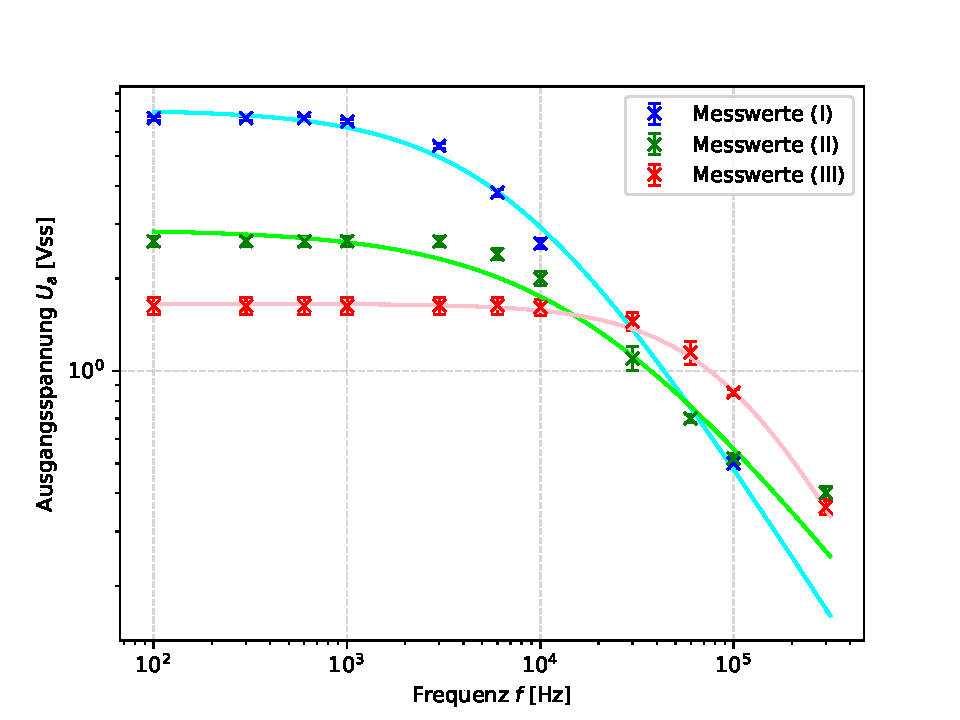
\includegraphics{graphics/plots/A2-1.pdf}}
    \caption{A2 - Frequenzgänge bei $R_g$ in Serie}
    \label{fig:A2_1}
\end{figure}

\begin{figure}[!p]
    \centering
    \resizebox{0.9\textwidth}{!}{
    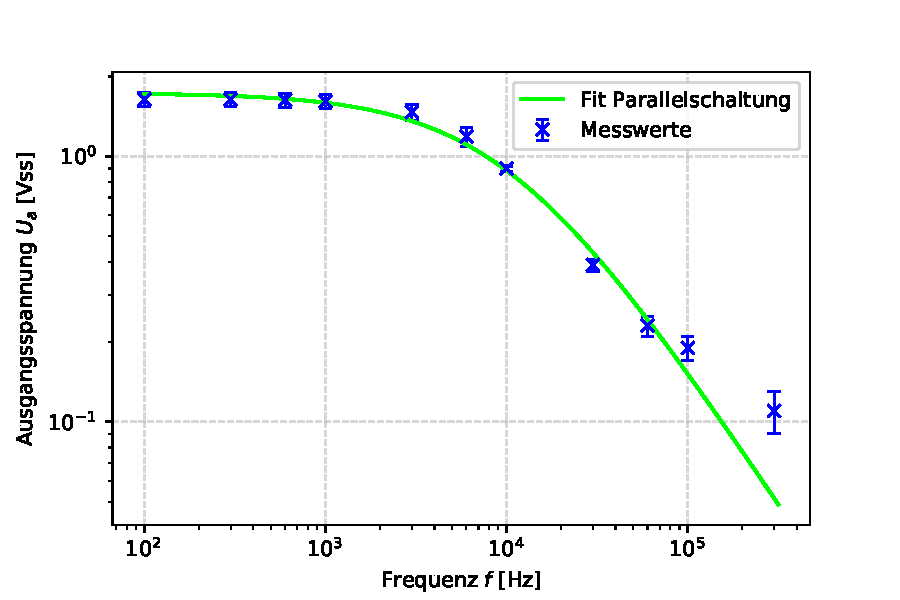
\includegraphics{graphics/plots/A2-2.pdf}}
    \caption{A2 - Frequenzgang bei $R_g$ Parallel}
    \label{fig:A2_2}
\end{figure}

\begin{figure}[!p]
    \centering
    \resizebox{0.9\textwidth}{!}{
    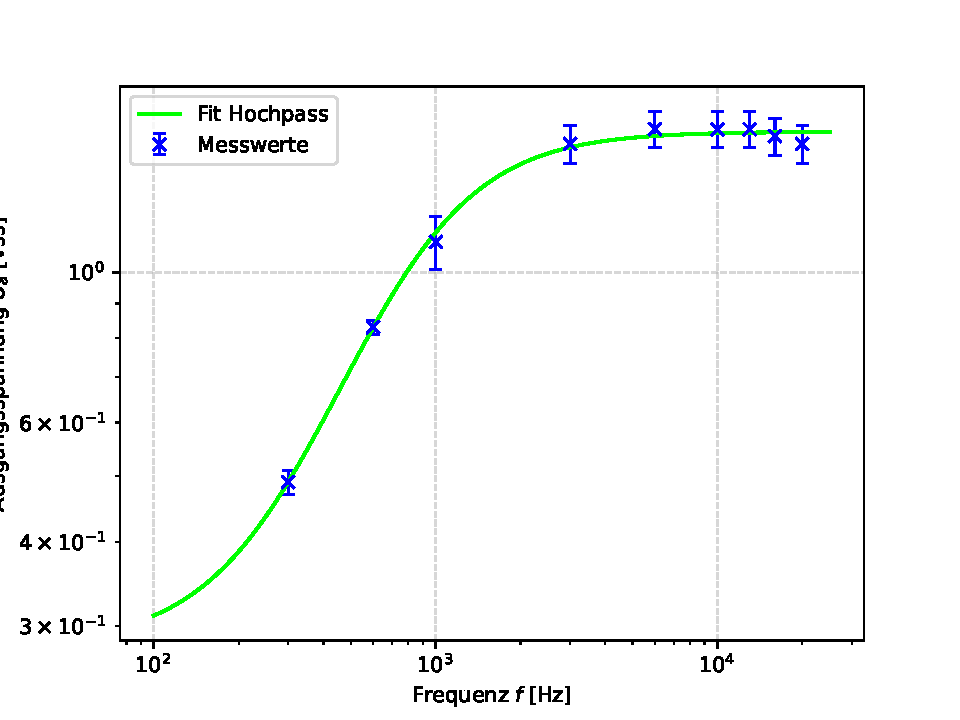
\includegraphics{graphics/plots/A2-3.pdf}}
    \caption{A2 - Frequenzgang bei $R_g$ in Serie und Eingangshochpassfilter}
    \label{fig:A2_3}
\end{figure}

\clearpage
\newpage
\subsection{Impulsverstärkung}

Wir möchten im letzten Teil qualitativ auf die verschiedenen Rückkopplungskonfigurationen und deren Auswirkungen auf das verwendete Rechtecksignal eingehen. 

Die ersten drei Bilder zeigen in unterschiedlichen Ausmaßen die gleichen Veränderungen des Ausgangssignals, was in Anbetracht der Tatsache, dass sich hier nur der Rückkopplungswiderstand ändert Sinn ergibt. Bei der ersten Konfiguration wird das Signal am meisten verstärkt, was anhand der gemessenen Spitze-Spitze-Spannung des Oszilloskops auf den Bildern zu erkennen ist, dafür werden hier aber auch die Kanten bei den einzelnen Signalen am stärksten abgeschwächt und das Signal ist nur noch ansatzweise als Rechtecksignal zu erkennen. Über das zweite bis zum dritten Signal hin werden nun die Verstärkung immer kleiner aber dafür die Kanten wieder umso schärfer. Insbesondere beim dritten Signal ist eine fast perfekte Rechteckform zu sehen, dafür liegt die Verstärkung aber auch nur bei etwa 1,6 im Vergleich zur ungefähr 22-fachen Verstärkung bei der ersten Konfiguration. Somit lässt sich festhalten, dass eine Erhöhung der Verstärkung über einen größeren Rückkopplungswiderstand gleichzeitig eine stärkere Formveränderung des Signals mit sich bringt.

Bei der vierten Konfiguration kommt zur Dritten eine zum Rückkopplungswiderstand parallel geschaltete Kapazität dazu. Die Verstärkung bleibt hierbei ungefähr gleich, jedoch werden die Kanten des Signals enorm abgeschwächt, etwa genau so viel wie bei der ersten Konfiguration. Eine parallel geschaltete Kapazität im Rückkopplungswiderstand sorgt also für eine stärkere Formveränderung des Signals bei gleichbleibender Verstärkung. 

Beim letzten Signal mit eingebautem Hochpassfilter beim Eingangssignal sowie parallelgeschaltetem Rückkopplungswiderstand und Kapazität lassen sich deutlich die Kombinationen der beiden Effekte beobachten. Die herausgefilterten niedrigen Frequenzen durch den Eingangshochpass sind deutlich daran zu erkennen, dass die 'Füllung' des Rechtecksignals fehlt und dieses somit in der Mitte abfällt. Ebenso ist wie im vierten Signal der unscharfe Anstieg der Kanten zu beobachten. Dennoch wird das Signal weiterhin insgesamt verstärkt, sogar etwas mehr als im vierten Fall, jedoch ist es nun überhaupt nicht mehr als Rechtecksignal zu erkennen. 

Insgesamt lässt sich also zusammenfassen, dass ein höherer Rückkopplungswiderstand das Signal verstärkt, es jedoch auch stärker umformt, eine parallel geschaltete Kapazität in der Rückkopplung die Verstärkung gleich lässt aber eine Verformung mit sich bringt und ein Hochpassfilter aufgrund der Filterung niedriger Frequenzen eine deutliche Formveränderung des Eingangssignals bewirkt. 






\clearpage
\newpage
%---------------PRÄSENTATION DER ENDERGEBNISSE---------------
\section{Zusammenfassung der Endergebnisse}

In diesem Versuch wurden die grundlegenden Eigenschaften und Verhaltensweisen eines Spannungsverstärkers untersucht. Zuerst untersuchten wir die Betriebsverstärkung des verwendeten Spannungsverstärkers bei verschiedenen Konfigurationen mit sowohl Gleich- als auch Wechselspannung. Hier wurden keine signifikanten Abweichungen von den theoretisch erwarteten Werten und Beobachtungen festgestellt, was teilweise jedoch auf die relativ hohen Fehler der Theoriewerte und die 10\%-ige Toleranz der Widerstände zurückzuführen war.

Im zweiten Versuchsteil untersuchten wir die Frequenzgänge bei verschiedenen Konfigurationen und konnten wie erwartet beobachten, dass sich die Verläufe für hohe Frequenzen einer in etwa gleich verlaufenden Leerlaufverstärkung annäherten. Ebenso zeigte die Messung bei zusätzlich parallel geschaltetem Widerstand ein ähnliches Verhalten und der Hochpassfilter ließ wie erwartet nur die hohen Frequenzen durch, während die Tieferen spürbar abgeschwächt wurden. 

Zum Schluss analysierten wir die Einflüsse verschiedener Konfigurationen auf die im Endeffekt erzielte Verstärkung und die Formveränderung des Ausgangssignals. Hier konnten wir feststellen, dass ein höherer Rückkopplungswiderstand eine stärkere Vergrößerung und Verformung erzielt, eine zusätzliche parallel geschaltete Kapazität die Verformung erhöht und ein Eingangshochpassfilter eine erwartete starke Verformung mit sich bringt. 



\newpage
%---------------ZUSAMMENFASSUNG UND DISKUSSION---------------
\section{Diskussion}

Insgesamt wurden in diesem Versuch sehr positive Ergebnisse erzielt. Alle Signifikanztests waren innerhalb insignifikanter Abweichungen und die erstellten Fits waren größtenteils zufriedenstellend. 

Dennoch sollen nun die bereits erwähnten hohen Toleranzen der Widerstände nochmal betont werden. Mit relativen Fehlern von 10\% waren diese so hoch, dass die theoretischen Betriebsverstärkungen Fehler von ca. 14\% aufwiesen und somit die Ergebnisse der Signifikanztests in ihrer Aussagekraft anzuzweifeln sind. Akkuratere Widerstände würden hier einen effektiveren Vergleich ermöglichen, wären aber auch anspruchsvoller in der Anwendung und erfordern strenger geregelte Umgebungsbedingungen, welche den Rahmen des Anfängerpraktikums gesprengt hätten. Somit sind die recht hohen Fehler ein dem Kontext dieses Versuches entsprechendes Resultat. 

Abgesehen davon waren die Messungen der anderen Versuchsteile in ihrer Genauigkeit immerzu ausreichend, um die qualitativen Beobachtungen aussagekräftig zu unterstützen. Die verwendeten Bauteile und Konfigurationen lieferten immer Ergebnisse, bei denen man die gewünschten Verläufe und Verhaltensweisen gut erkennen konnte, sodass aussagekräftige Ergebnisse erzielt werden konnten.

Zusammenfassend lässt sich also sagen, dass in diesem Versuch Ergebnisse erzielt wurden, die im Kontext des Physikalischen Anfägerpraktikums durchaus zufriedenstellend sind und der durch den Aufbau bedingten Genauigkeit mehr als genügten. Sowohl die qualitativen als auch die quantitativen Teile ergaben mit der Theorie und untereinander vereinbare Ergebnisse, die für ein grundlegendes Verständnis der Thematik und somit eine angemessene Einführung sorgten.







 
\newpage
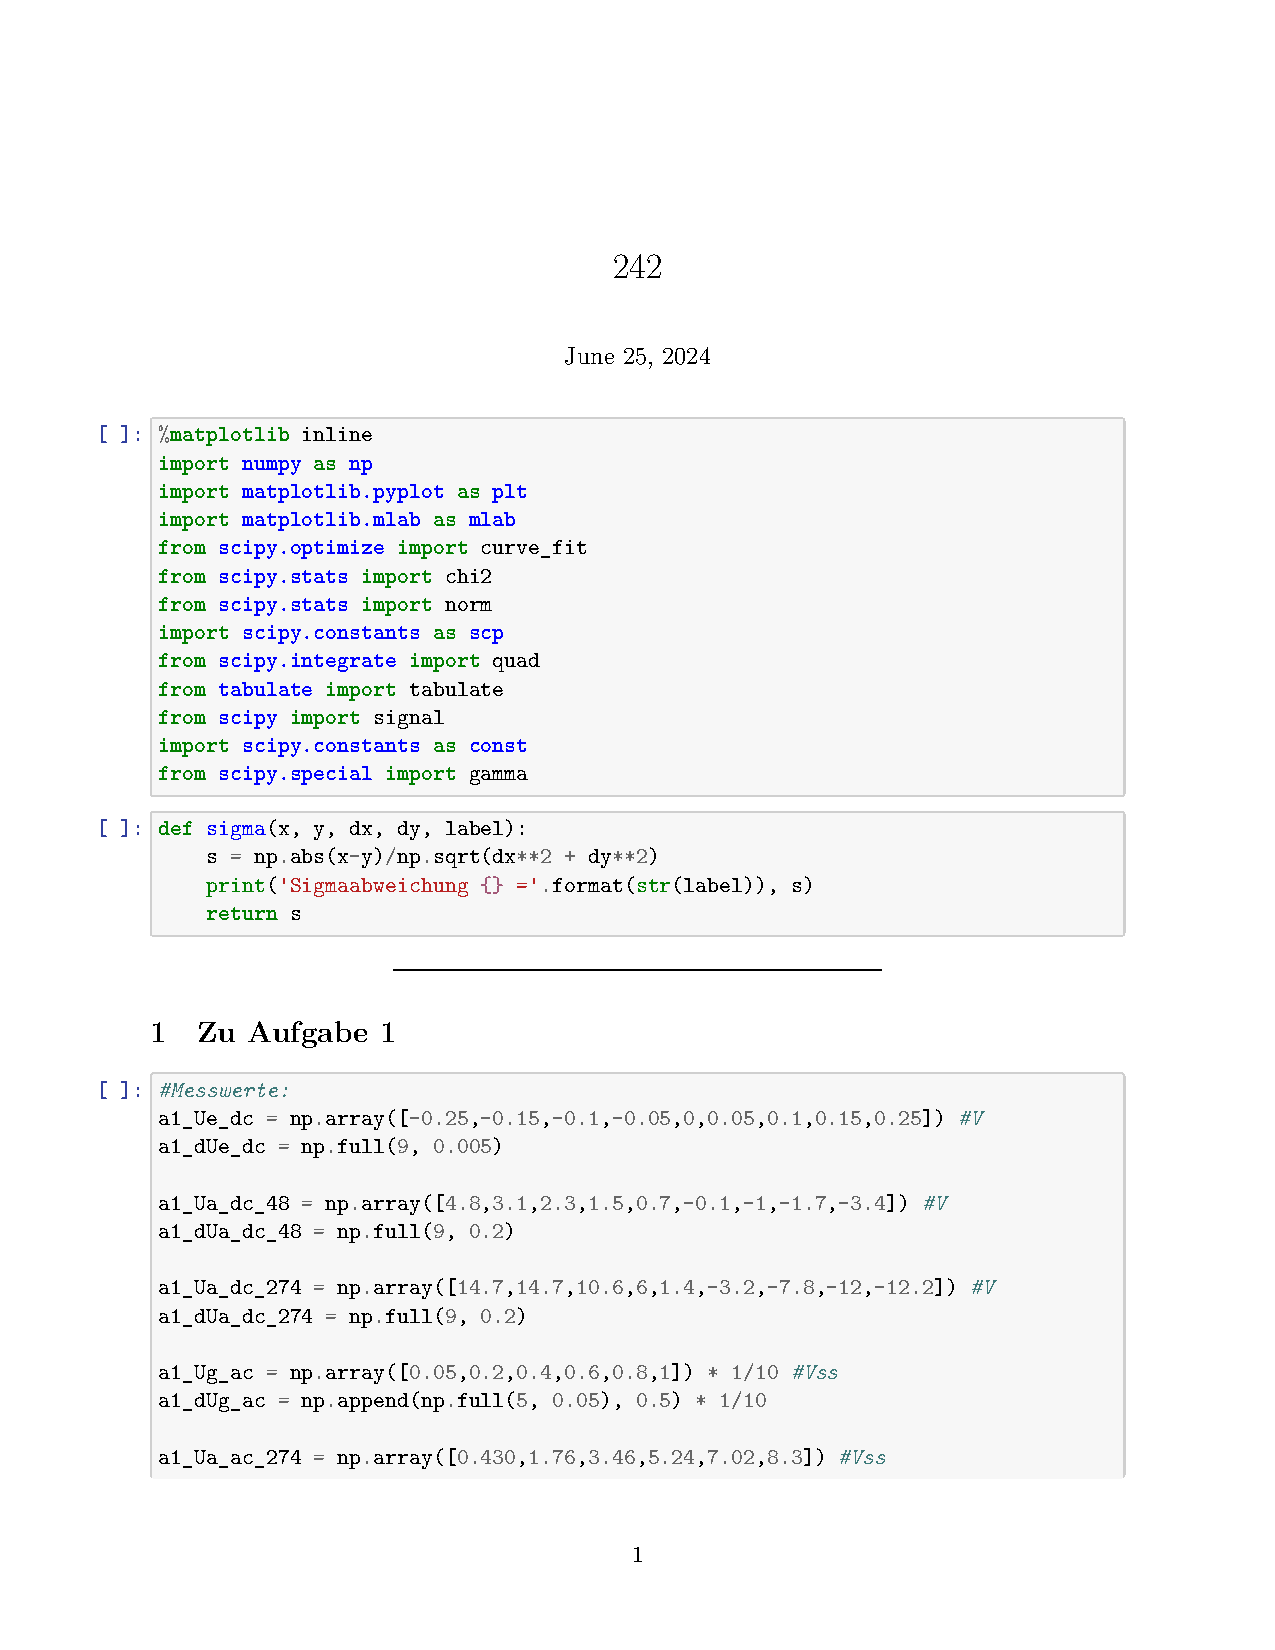
\includepdf[pagecommand=\invisiblesection{Python-Code},scale=0.8,pages=1]{242.pdf}
\includepdf[pagecommand={},scale=0.8,pages=2-last]{242.pdf}

\end{document}

